%%%%%%%%%%%%%%%%%%%%%%%%%%%%%%%%%%%%%%%%%
% Masters/Doctoral Thesis 
% LaTeX Template
% Version 2.5 (27/8/17)
%
% This template was downloaded from:
% http://www.LaTeXTemplates.com
%
% Version 2.x major modifications by:
% Vel (vel@latextemplates.com)
%
% This template is based on a template by:
% Steve Gunn (http://users.ecs.soton.ac.uk/srg/softwaretools/document/templates/)
% Sunil Patel (http://www.sunilpatel.co.uk/thesis-template/)
%
% Template license:
% CC BY-NC-SA 3.0 (http://creativecommons.org/licenses/by-nc-sa/3.0/)
%
%%%%%%%%%%%%%%%%%%%%%%%%%%%%%%%%%%%%%%%%%

%----------------------------------------------------------------------------------------
%	PACKAGES AND OTHER DOCUMENT CONFIGURATIONS
%----------------------------------------------------------------------------------------

\documentclass[
11pt, % The default document font size, options: 10pt, 11pt, 12pt
oneside, % Two side (alternating margins) for binding by default, uncomment to switch to one side
english, % ngerman for German
singlespacing, % Single line spacing, alternatives: onehalfspacing or doublespacing
%draft, % Uncomment to enable draft mode (no pictures, no links, overfull hboxes indicated)
%nolistspacing, % If the document is onehalfspacing or doublespacing, uncomment this to set spacing in lists to single
liststotoc, % Uncomment to add the list of figures/tables/etc to the table of contents
toctotoc, % Uncomment to add the main table of contents to the table of contents
%parskip, % Uncomment to add space between paragraphs
%nohyperref, % Uncomment to not load the hyperref package
headsepline, % Uncomment to get a line under the header
%chapterinoneline, % Uncomment to place the chapter title next to the number on one line
%consistentlayout, % Uncomment to change the layout of the declaration, abstract and acknowledgements pages to match the default layout
]{MastersDoctoralThesis} % The class file specifying the document structure
\usepackage{amsmath}
\usepackage{bm}
\usepackage{algorithm2e}
\RestyleAlgo{ruled}
\usepackage[utf8]{inputenc} % Required for inputting international characters
\usepackage[T1]{fontenc} % Output font encoding for international characters

\usepackage{mathpazo} % Use the Palatino font by default
\usepackage{float}
\usepackage[backend=biber,style=alphabetic, sorting=nyvt]{biblatex}

\addbibresource{references.bib} % The filename of the bibliography

\usepackage[autostyle=true]{csquotes} % Required to generate language-dependent quotes in the bibliography

% Custom packages
\usepackage{blindtext}
\usepackage{bbm}
\usepackage{amssymb}
\usepackage{hyperref}
\usepackage{epigraph} 
\usepackage{xstring}

%----------------------------------------------------------------------------------------
%	CUSTOM MATH COMMANDS
%----------------------------------------------------------------------------------------
\newcommand{\bb}[1]{\mathbb{#1}}
\newcommand{\LagDerivative}[2][t]{\frac{\operatorname{D} #2}{\operatorname{D} #1}}
\newcommand{\PartialDerivative}[2][t]{\frac{\partial #2}{\partial #1}}
\newcommand{\vect}[1]{\mathbf{#1}}
\newcommand{\tensor}[1]{\underline{\underline{\bm{#1}}}}
\newcommand{\WIJ}{W_{h, ij}}
\newcommand{\DWIJ}{\nabla_{i} W_{h, ij}}
\newcommand{\VIJ}{\vect{v}_{ij}}
\newcommand{\RIJ}{\vect{r}_{ij}}
\newcommand{\RtwoIJ}[1][2]{|\vect{r}_{ij}|^{#1}}
\newcommand{\MachineEpsilon}{\bm{\xi}}
\newcommand{\EncAngBrk}[2][]{#1\langle #2 #1\rangle}
\newcommand{\RAProp}[1]{\EncAngBrk{#1}}
\newcommand{\FrobeniusInnerProduct}[2]{\EncAngBrk{\tensor{#1}, \tensor{#2}}}
\newcommand{\FrobeniusNorm}[1]{||\tensor{#1}||_F}
\newcommand{\BasisVect}[1][i]{\hat{\vect{e}}_{#1}}
\newcommand{\HalfFrac}{\frac{1}{2}}
\newcommand{\Vol}[1][V]{\mathcal{#1}}
\newcommand{\Vorticity}{\bm{\omega}}
\newcommand{\Boundary}{\bm{\Omega}}
\newcommand{\WaveNumber}{\mathrm{k}}
\newcommand{\WaveNumberVector}{\vect{k}}
\newcommand{\TildeR}{\widetilde{\vect{r}}}
\newcommand{\TildeV}{\widetilde{\vect{v}}}
\newcommand{\TildeDeltaV}{\delta\TildeV}
\newcommand{\TildeRho}{\widetilde{\rho}}
\newcommand{\TildeP}{\widetilde{P}}
\newcommand{\IntRThreeAndT}{\int_{\mathbf{R}^3} \int_{-\infty}^{\infty}}





%----------------------------------------------------------------------------------------
%	MARGIN SETTINGS
%----------------------------------------------------------------------------------------

\geometry{
	paper=a4paper, % Change to letterpaper for US letter
	inner=2.5cm, % Inner margin
	outer=3.8cm, % Outer margin
	bindingoffset=.5cm, % Binding offset
	top=1.5cm, % Top margin
	bottom=1.5cm, % Bottom margin
	%showframe, % Uncomment to show how the type block is set on the page
}

%----------------------------------------------------------------------------------------
%	THESIS INFORMATION
%----------------------------------------------------------------------------------------

\thesistitle{A Comparative Study of Turbulence Modelling for Smoothed Particle Hydrodynamics} % Your thesis title, this is used in the title and abstract, print it elsewhere with \ttitle
\supervisor{Prof. Prabhu Ramachandran} % Your supervisor's name, this is used in the title page, print it elsewhere with \supname
\examiner{} % Your examiner's name, this is not currently used anywhere in the template, print it elsewhere with \examname
\degree{ } % Your degree name, this is used in the title page and abstract, print it elsewhere with \degreename
\author{K T Prajwal Prathiksh} % Your name, this is used in the title page and abstract, print it elsewhere with \authorname
\addresses{} % Your address, this is not currently used anywhere in the template, print it elsewhere with \addressname

\subject{Biological Sciences} % Your subject area, this is not currently used anywhere in the template, print it elsewhere with \subjectname
\keywords{Fluid Mechanics, Turbulence Modelling, Smoothed Particle Hydrodynamics, Reynolds Averaging, Large Eddy Simulation, Lagrangian Averaging, Coherent Structures} % Keywords for your thesis, this is not currently used anywhere in the template, print it elsewhere with \keywordnames
\university{{Indian Institute of Technology Bombay}} % Your university's name and URL, this is used in the title page and abstract, print it elsewhere with \univname
\department{{Department of Aerospace Engineering}} % Your department's name and URL, this is used in the title page and abstract, print it elsewhere with \deptname
\group{\href{http://researchgroup.university.com}{ }} % Your research group's name and URL, this is used in the title page, print it elsewhere with \groupname
\faculty{\href{http://faculty.university.com}{ }} % Your faculty's name and URL, this is used in the title page and abstract, print it elsewhere with \facname

\AtBeginDocument{
\hypersetup{pdftitle=\ttitle} % Set the PDF's title to your title
\hypersetup{pdfauthor=\authorname} % Set the PDF's author to your name
\hypersetup{pdfkeywords=\keywordnames} % Set the PDF's keywords to your keywords
}

\begin{document}

\frontmatter % Use roman page numbering style (i, ii, iii, iv...) for the pre-content pages

\pagestyle{plain} % Default to the plain heading style until the thesis style is called for the body content

%----------------------------------------------------------------------------------------
%	TITLE PAGE
%----------------------------------------------------------------------------------------

\begin{titlepage}
\begin{center}


\begin{figure}[H]
\centering

\includegraphics[scale=0.12]{Figures/iitb-logo}
\end{figure}

\vspace*{.06\textheight}
{\scshape\LARGE \univname\par}\vspace{1.5cm} % University name
\textsc{\Large AE 593 - Dual Degree Project I }\\[0.5cm] % Thesis type

\HRule \\[0.4cm] % Horizontal line
{\huge \bfseries \ttitle\par}\vspace{0.4cm} % Thesis title
\HRule \\[1.5cm] % Horizontal line
 
\begin{minipage}[t]{0.4\textwidth}
\begin{flushleft} \large
\emph{Submitted By:}\\
{\authorname \\ 180010027} % Author name - remove the \href bracket to remove the link
\end{flushleft}
\end{minipage}
\begin{minipage}[t]{0.4\textwidth}
\begin{flushright} \large
\emph{Supervisor:} \\
{\supname} % Supervisor name - remove the \href bracket to remove the link  
\end{flushright}
\end{minipage}\\[1cm]
 
\vfill

\large \textit{Report submitted in fulfillment of the requirements for Dual Degree Project I}\\[0.3cm] % University requirement text
\textit{in the}\\[0.05cm]
\groupname\\\deptname\\[2cm] % Research group name and department name
 
\vfill

{\large \today}\\[2cm] % Date
%\includegraphics{Logo} % University/department logo - uncomment to place it
 
\vfill
\end{center}
\end{titlepage}



%----------------------------------------------------------------------------------------
%	ABSTRACT PAGE
%----------------------------------------------------------------------------------------

\begin{abstract}
\addchaptertocentry{\abstractname} % Add the abstract to the table of contents
Turbulence modelling is a challenging problem, particularly for a Lagrangian method such as Smoothed Particle Hydrodynamics (SPH) which lacks the years of theoretical and practical research that conventional CFD solvers based on FEM/FVM enjoy. However, work based on translating existing Eulerian-based turbulence methods to SPH and Lagrangian-specific models has started making inroads in the general understanding of the topic in an SPH setting. Ultimately, a rigorous and robust model can be devised, which is well-suitable to a wide variety of $2D$ and $3D$ problems.
This project aims to survey and review the state-of-the-art turbulence models that SPH offers and help subsequently provide a comparative analysis detailing the advantages and limitations of these models.
It also intends to extend the best-equipped models to robust and accurate SPH schemes and incorporate some of the latest developments in the field of SPH to refine further the machinery required to model turbulence.

\textbf{Keywords:} \keywordnames



\end{abstract}


%----------------------------------------------------------------------------------------
%	LIST OF CONTENTS/FIGURES/TABLES PAGES
%----------------------------------------------------------------------------------------

\tableofcontents % Prints the main table of contents

\listoffigures % Prints the list of figures

\chapter*{List of Symbols}

\addcontentsline{toc}{chapter}{List of Symbols}
\setlength{\tabcolsep}{10pt} % Default value: 6pt - Column Spacing
\renewcommand{\arraystretch}{1.7} % Default value: 1 - Row Spacing

%TODO Increase size of Header

% Please add the following required packages to your document preamble:
% \usepackage{longtable}
% Note: It may be necessary to compile the document several times to get a multi-page table to line up properly
\begin{longtable}{ll}
\textbf{Symbol}         & \textbf{Description}              \\
\endfirsthead
%
\multicolumn{2}{c}%
{{\bfseries Table \thetable\ continued from previous page}} \\
\textbf{Symbol}         & \textbf{Description}              \\
\endhead
%
$\vect{a}$              & Vector Field                      \\
$\tensor{A}$            & Second-rank Tensor Field          \\
$\BasisVect$            & $i^{th}$ Basis                    \\
$\otimes$               & Tensor Product                    \\
$\LagDerivative{()}$    & Lagrangian Derivative             \\
$\FrobeniusInnerProduct{A}{B}$ & Frobenius Inner Product of $\tensor{A}$ and $\tensor{B}$                                    \\
$\FrobeniusNorm{A}$            & Frobenius Norm of $\tensor{A}$ $( = \sqrt{\FrobeniusInnerProduct{\tensor{A}}{\tensor{A}}})$ \\
$\nabla^2$              & Laplacian Operator                \\
$\Delta ()$             & Component-wise Laplacian Operator \\
$(1 - \alpha^2 \Delta)$ & Helmholtz Operator                \\
$i$                     & Reference Particle                \\
$j$                     & Neighbouring Particle             \\
$(...)_{i}$             & Property of $i^{th}$ SPH particle \\
$(...)_{j}$             & Property of $j^{th}$ SPH particle \\
$(...)_{ij}$            & $(...)_{i} - (...)_{j}$           \\
$t$                     & Time                              \\
$\vect{r}$              & Position $=(x, y, z)$             \\
$\vect{v}$              & Velocity $=(v_x, v_y, v_z)$       \\
$m$                     & Mass                              \\
$P$                     & Pressure                          \\
$\rho$                  & Density                           \\
$(...)_0$                      & Initial Condition ($(t=0$ of Specified Property                                             \\
$\Delta t$              & Time Step                         \\
$\Delta x$              & Inter Particle Spacing            \\
$\delta (x)$            & Dirac Delta Function              \\
$W_{h}$                 & SPH Interpolating Kernel          \\
$h$                     & Kernel Smoothing Length           \\
$\WIJ$                  & $W(|\RIJ|, h)$                    \\
$\DWIJ$                        & $\nabla_i W(\RIJ,h) = \frac{\RIJ}{\RtwoIJ[]} \PartialDerivative[r_i]{\WIJ}$                 \\
$\Vol_i$                & Volume of $i^{th}$ SPH particle   \\
$\varphi_i$                    & Particle Density of $i^{th}$ SPH particle                                                   \\
$\vect{F}$              & External Body Force               \\
$\nu$                   & Kinematic Viscosity               \\
$\eta$                  & Dynamic Viscosity $(=\nu \rho)$   \\
$\MachineEpsilon$       & Machine Epsilon                   \\
$M_o$                   & Reference Mass                    \\
$P_o$                   & Reference Pressure                \\
$\rho_o$                & Reference Density                 \\
$c_s$                   & Speed of Sound                    \\
$\gamma$                & Exponent - Equation of State      \\
$\Vorticity$                   & Vorticity $(=\nabla \times \vect{v})$                                                       \\
$\nu_t$                 & Turbulent Eddy Viscosity          \\
$\tensor{S}$                   & Strain-Rate Tensor $(=[1/2][\nabla \vect{v} + \nabla \vect{v}^T])$                          \\
$\tensor{R}$                   & Rate of Rotation Tensor $(=[1/2][\nabla \vect{v} - \nabla \vect{v}^T])$                     \\
$\epsilon$              & Turbulent Dissipation Rate        \\
$k$                     & Turbulent Kinetic Energy          \\
$\tensor{\tau}$         & Stress Tensor                     \\
$C_s $                  & Smagorinsky Constant              \\
$u_{max}$               & Maximum Particle Velocity         \\
$\varepsilon$           & Smoothing Parameter (XSPH)        \\
$\WaveNumber$           & Wave Number                      
\end{longtable}

%\listoftables % Prints the list of tables

%----------------------------------------------------------------------------------------
%	ABBREVIATIONS
%----------------------------------------------------------------------------------------


%----------------------------------------------------------------------------------------
%	PHYSICAL CONSTANTS/OTHER DEFINITIONS
%----------------------------------------------------------------------------------------

% \begin{constants}{lr@{${}={}$}l} % The list of physical constants is a three column table

% % The \SI{}{} command is provided by the siunitx package, see its documentation for instructions on how to use it
% \textcolor{red}{FILL IN Later!!}\\

% Sea-level gravitational acceleration & $g_{0}$ & \SI{9.81}{\meter\per\second\squared}\\
% Planck's constant & $h$ & \SI{6.62607004e-34}{\meter\squared\kg\per\second}\\
% Boltzmann constant& $k$ &\SI{1.38064852e-23}{\meter\squared\kg\per\second\squared\per\kelvin}\\
% %Constant Name & $Symbol$ & $Constant Value$ with units\\

% \end{constants}

%----------------------------------------------------------------------------------------
%	SYMBOLS
%----------------------------------------------------------------------------------------

% \begin{symbols}{lll} % Include a list of Symbols (a three column table)

% $r$ & radial distance & \si{\meter} \\
% $\theta$ & azimuthal angle & \si{\radian} \\
% $z$ & axial distance & \si{\meter} \\
% $\#$ & number & - \\
% $r$ & radial direction & \si{\meter} \\
% $r$ & radial direction & \si{\meter} \\
% $r$ & radial direction & \si{\meter} \\


% \end{symbols}


%----------------------------------------------------------------------------------------
%	THESIS CONTENT - CHAPTERS
%----------------------------------------------------------------------------------------

\mainmatter % Begin numeric (1,2,3...) page numbering

\pagestyle{thesis} % Return the page headers back to the "thesis" style

% Include the chapters of the thesis as separate files from the Chapters folder
% Uncomment the lines as you write the chapters

\chapter{Introduction} % Main chapter title
\label{Chapter1}

\epigraph{Turbulence is the most important unsolved problem of classical physics.}{\textit{Richard Feynman}}

Turbulent flows have long been a phenomenon that is surprisingly easy to detect and observe in the natural world but unmistakably challenging to understand and model in sufficient detail, unlike other problems in classical physics.
The fundamental aspects of turbulent flow consisting of eddies of various length scales had long been observed, as recorded by Leonardo Da Vinci's $16^{th}$ century diagrams of water flow in streams and channels from the  \parencite{Colagrossi2021DaVinci}.
It took the work of Osborne Reynolds and William Thomson (Lord Kelvin) from the late $19th$ century for the scientific community to demarcate the separation between the laminar and turbulent flow. However, further strides in the field have remained arduous despite the Navier-Stokes (NS) equations being written down in the early $19^{th}$ century. There is consensus that this remarkable failure of some of the greatest scientific minds in providing an intricate understanding of turbulence points to an inadequacy of the mathematical tools we have at our disposal. Even the current machinery cannot deal with the strong non-linearity of the equations coupled with the characteristic tendency of flows to degenerate into some form of instability.

\begin{figure}[h!]
    \centering
    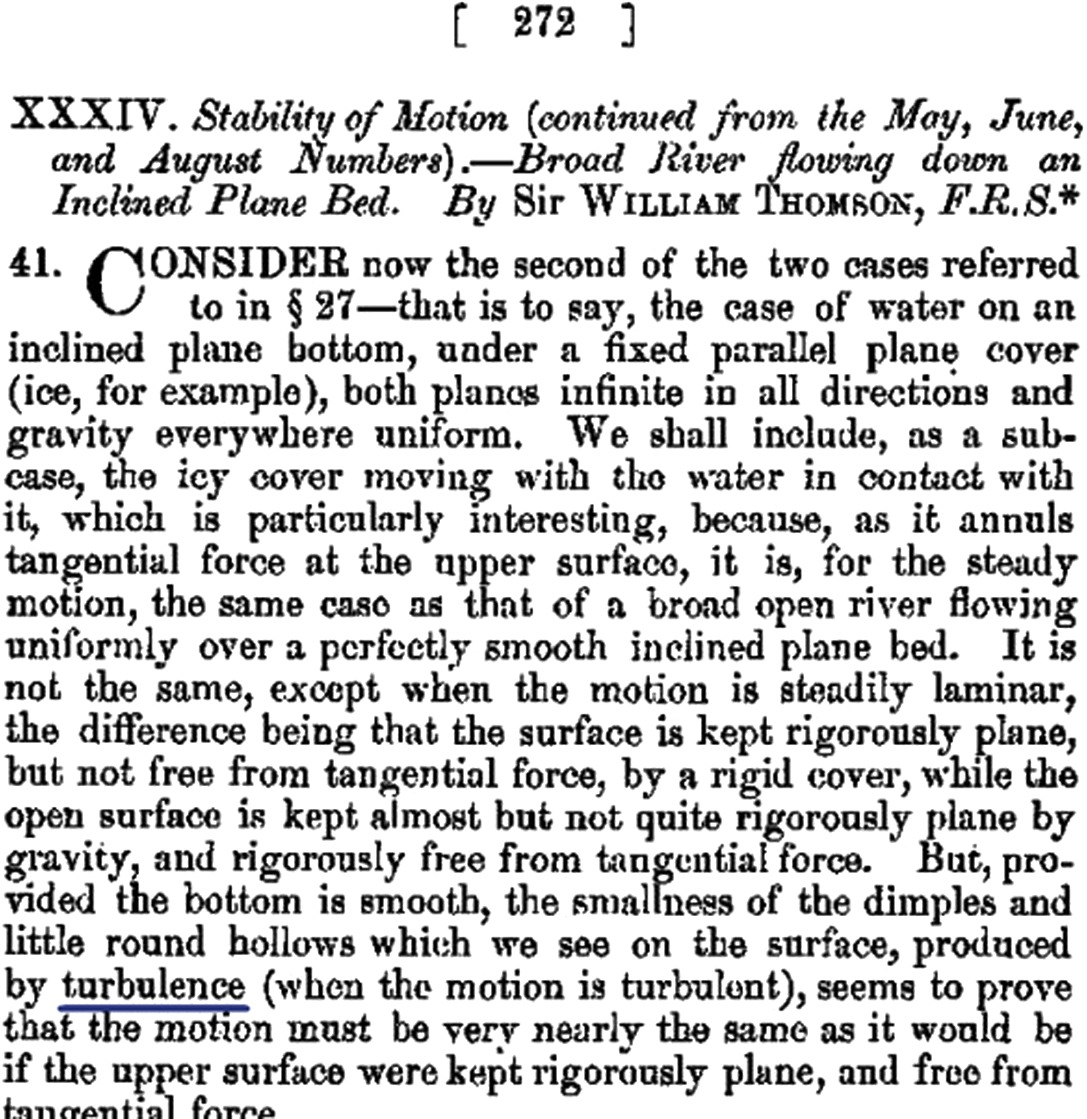
\includegraphics{Figures/research_papers/schmitt2017turbulence-fig-1.jpg}
    \caption{A scanned copy of a part of the first page of the 1887 paper by William Thomson, where the word \textit{'turbulence'}, as a noun, is first introduced. Ref: \parencite{schmitt2017turbulence}}
    \label{fig:schmitt2017turbulence-fig-1}
\end{figure}

Turbulence is caused by excessive kinetic energy in parts of a fluid flow that can overcome the damping effect of the fluid's viscosity. Its onset can be predicted by the dimensionless Reynolds number, which is the ratio of kinetic energy to viscous damping in a fluid flow. 

The criteria for defining a flow as turbulent are varied and ambiguous since there is no explicit definition for it. However, the most often used criteria for qualifying a flow as turbulent is given below \parencite{sagaut2002statistical}:
\begin{itemize}
    \item random character of the spatial and temporal fluctuations of the velocities, which reflect the existence of finite characteristic scales of statistical correlation;
    \item velocity field is three-dimensional and rotational;
    \item various modes are strongly coupled, which is reflected in the non-linearity of the NS equations;
    \item large mixing capacity due to the agitation induced by the various scales;
    \item chaotic character of the solution, which exhibits a powerful dependency on the initial condition and boundary conditions.
\end{itemize}

\section{Smoothed Particle Hydrodynamics}
Smoothed particle hydrodynamics (SPH) is a technique for problem-solving in \textit{Computational Continuum Dynamics} (CCD). This technique approximates numerical solutions of the equations of fluid dynamics by replacing the fluid with a set of particles. The equations of motion and properties of these particles are determined from the continuum equations of fluid dynamics. They are subsequently discretised based on the particles' interpolant data. The interpolant can be constructed using analytical functions, and spatial derivatives of the interpolated quantities can then be found using ordinary calculus. There is no need to use a grid, and the description of free surfaces, however complicated, is trivial.

Therefore, this \textit{Lagrangian} based particle formulation uses no background spatial mesh. Since there is no mesh to distort, the method can handle large deformations in a pure Lagrangian frame. Thus, material interfaces can be modelled naturally, and complex constitutive behaviour can be implemented relatively quickly. This allows SPH to have diverse and fascinating applications in various domains that extend beyond the astrophysical and cosmological problems it was initially designed to tackle.

\section{Project Motivation \& Objectives}
Despite the success of SPH in simulating transient flows, a robust or rigorous model of turbulence does not seem to exist. Some of the models in use cannot be generalised to a wide variety of turbulence-based problems or scaled to $3D$-flows.
This limits SPH's applicability in turbulent flows where conventional FEM/FVM-based CFD solvers have the upper hand, owing to their sophisticated models.

This project aims to survey and review the current state of the art regarding turbulence modelling in SPH and subsequently provide a framework to help establish the advantages and limitations of such models, using a comparative analysis between the major class of models.
After that, it is intended to extend the most well-equipped models to robust and accurate SPH schemes (which might not have been the case in the author/s original work). Such an exercise is expected to either improve the original model or expose any underlying limitations in its assumptions or discretisation.

\section{Report Structure}
The report is structured to present the turbulence models developed for SPH in Chapter \ref{Chapter2}. Here, the models have been categorised by the fundamental ideas on which they were based. Subsequently, research on analysing turbulence through standard benchmarks problems and methods of quantifying turbulence data is presented in Chapter \ref{Chapter3}.
Finally, the project conclusion and future work for Stage - II of the Dual Degree Project are presented in Chapter \ref{Chapter4}. 

\chapter{Turbulence Modelling} % Main chapter title
\label{Chapter2}

\section{Viscosity-Based Models}
Violeau et al. \parencite{VIOLEAU2002} were amongst the early pioneers who tried to incorporate a turbulence model in SPH. They came up with two techniques to tackle the problem of turbulence in a Lagrangian framework, which so far had been neglected till then in research, namely, the eddy viscosity model and a generalised Langevin model. For each of their techniques, they considered the following equation of state \ref{eq:violeau-eos}, continuity equation \ref{eq:violeau-continuity} and momentum equation \ref{eq:violeau-mom}, based on the work of \parencite{Monaghan1992}:

\begin{equation}
	P_i = B \Bigg[ \bigg( \frac{\rho_i}{\rho_0} \bigg)^{\gamma} - 1 \Bigg], B = \frac{\rho_0 c_s^2}{\gamma}
	\label{eq:violeau-eos}
\end{equation}
\begin{equation}
	\LagDerivative{\rho_i} = \sum_j m_j \VIJ \cdot \DWIJ
	\label{eq:violeau-continuity}
\end{equation}
\begin{equation}
	\LagDerivative{\vect{v}_i} = - \sum_j m_j \bigg( \frac{P_i}{\rho_i^2} + \frac{P_j}{\rho_j^2} + \Pi_{ij} \bigg) \DWIJ + \vect{F}_i
	\label{eq:violeau-mom}
\end{equation}

Where the viscous term is defined as:
\begin{equation}
	\Pi_{ij} = - \frac{16\nu}{\rho_i + \rho_j} \frac{\VIJ \cdot \RIJ}{\RtwoIJ + \MachineEpsilon^2} 
	\label{eq:violeau-diffusion-term}
\end{equation}

\subsection{Eddy Viscosity Model}
\label{sec:eddy-visc-model}

The eddy viscosity model was devised as a first-order closure model, which consisted of a relationship between the Reynolds stress tensor and the mean velocity gradients. Therefore, the momentum equation is similar to the momentum equation, except that the kinematic viscosity is replaced by the eddy viscosity $(\nu_t)$, and the velocities are Reynolds-averaged. In the SPH formalism, the diffusion term occurring is therefore defined as given in \ref{eq:violeau-turbulent-diffusion-term}, with the eddy viscosity defined according to \ref{eq:violeau-eddy-viscosity}.
\begin{equation}
	\widetilde{\Pi}_{ij} = -8 \frac{\nu_{t, i} + \nu_{t, j}}{\rho_i + \rho_j} \frac{\RAProp{\vect{v}}_{ij} \cdot \RIJ }{\RtwoIJ + \MachineEpsilon^2}
	\label{eq:violeau-turbulent-diffusion-term}
\end{equation}
\begin{equation}
	\nu_t = L_m^2 \FrobeniusNorm{S} = L_m^2 \sqrt{\FrobeniusInnerProduct{S}{S}}
	\label{eq:violeau-eddy-viscosity}
\end{equation}

Where $\RAProp{\vect{v}}$ is Reynolds-averaged velocity, and $L_m$ refers to the mixing length scales. The SPH formulation for the mean velocity gradients are given in \ref{eq:violeau-mean-velocity-gradient}.

\begin{equation}
	\nabla \RAProp{\vect{v}}_i = - \frac{1}{\rho_i} \sum_j m_j \RAProp{\vect{v}}_{ij} \otimes \DWIJ
	\label{eq:violeau-mean-velocity-gradient}
\end{equation}

On simulating Poiseuille flow for a high Reynolds number case, the authors could show that the velocity profile showed only a slight discrepancy with theory, with the expected log-law profile near the walls \ref{fig:violeau2002-eddy-viscosity-result}. This indicated that the model is appropriate for turbulent mixing problems or for cases involving spatially-varying viscosity while restricted to shear flows.

\begin{figure}[h!]
	\centering
	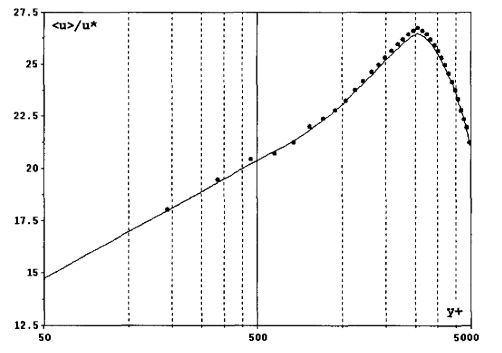
\includegraphics{Figures/research_papers/violeau2002-eddy-viscosity-result.png}
	\caption{Turbulent Poiseuille flow in a pipe $(Re = 64e3)$ modelled using the eddy viscosity model. Computed mean velocity profiles after $(t=1s)$ (solid circles), against theory (solid line). Ref: \parencite{VIOLEAU2002}}
	\label{fig:violeau2002-eddy-viscosity-result}
\end{figure}

\subsection{Generalized Langevin Model}
Violeau et al. also considered a stochastic approach, where the main idea is built on the concept of prescribing particle velocities as a random process, with properties fulfilling the theoretical turbulence hypotheses \parencite{pope1994lagrangi}. Hence, came about the Generalised Langevin model (GLM), where the particle acceleration is defined as:
\begin{equation}
	d\vect{v} = -\frac{1}{\rho} \nabla \RAProp{P} + \tensor{G}(\vect{v} - \RAProp{\vect{v}})dt + \sqrt{C_0 \epsilon dt}\vect{\xi}
	\label{eq:violeau-glm-particle-accel}
\end{equation}

Where $\Vec{\xi}$ is a random vector statistically non-correlated with velocities. The closure for this model was defined by specifying $\tensor{G}$ as:
\begin{equation}
	\tensor{G} = \HalfFrac C_1 \frac{\epsilon}{k}\tensor{I} + C_2 \nabla \RAProp{\vect{v}}
\end{equation}

Where $(k)$ is the turbulent kinetic energy, $(E)$ the dissipation rate, and $(C_i)$ being constants - $(C_1=1.8, C_2=0.6)$.
By modelling turbulence as GLM in SPH, the momentum equation derived was given by:
\begin{equation}
	\LagDerivative{\vect{v}_i} = -\sum_j m_j \bigg( \frac{\RAProp{P}_i}{\rho_i^2} + \frac{\RAProp{P}_j}{\rho_j^2} \bigg) \DWIJ - \HalfFrac C_1 \frac{\epsilon_i}{k_i} \vect{v}'_i + C_2 \nabla \RAProp{\vect{v}}_i \cdot \vect{v}'_i + \sqrt{\frac{C_0 \epsilon_i}{\delta t}} \Vec{\xi}_i
	\label{eq:violeau-mom-glm}
\end{equation}
\begin{equation}
	\RAProp{\vect{v}} = \sum_j \frac{m_j}{\rho_j}\vect{u}_j W_h (\vect{r}_j)
	\label{eq:violeau-ra-vel}
\end{equation}

Where the fluctuations are defined as $\vect{v}' = \vect{v} - \RAProp{\vect{v}}$, and the local values of turbulent kinetic energy and dissipation rate are:
\begin{align}
	\epsilon_i = 2 \nu_{t, i} + 
	\FrobeniusNorm{S_i}^2 \\
	k_i = \frac{\epsilon_i \nu_{t, i}}{C_{\mu}}, C_{\mu} = 0.009
	\label{eq:violeau-k-eps}
\end{align}

It is to be noted that the authors did not estimate the dissipation rate through the proper velocity gradients since the fluctuations of random velocities do not reproduce the small eddies.
The same test case as mentioned in \ref{sec:eddy-visc-model} was considered for the performance of GLM. 
The authors observed large fluctuations. They attributed the discrepancy to the mean operator being redefined as given by \ref{eq:violeau-ra-vel} instead of being a Reynolds average. In fact, by redefining the mean operator in such a fashion, they appeared to have constructed a rudimentary LES filter. 
As observed in \ref{fig:violeau2002-GLM-result}, the fluctuations have an order of magnitude of $k^{1/2}$. However, as claimed by the authors, unlike the eddy viscosity model, the GLM method can be used for different flows instead of being restricted to only shear flows.
\begin{figure}[h!]
	\centering
	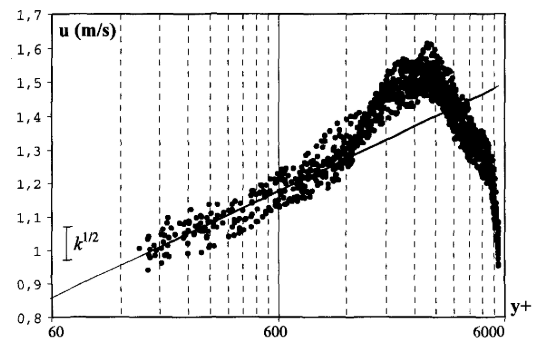
\includegraphics{Figures/research_papers/violeau2002-GLM-result.png}
	\caption{Turbulent Poiseuille flow in a pipe $(Re = 64e3)$ modelled using the generalised Langevin model. Computed mean velocity profiles after $(t=1s)$ (solid circles), against theory (solid line). Ref: \parencite{VIOLEAU2002}}
	\label{fig:violeau2002-GLM-result}
\end{figure}


\section{mSPH}
Adami et al. \parencite{Adami2012} devised a model built on their observation of SPH simulations, wherein the absence of viscosity in typical SPH formulations produced purely noisy particle motion. At finite viscosities, the method would over-predict dissipation. Hence to counter this, they essentially "modified" (hence the name: Modified SPH [mSPH]) the momentum equation and the equation of state to advect the particles in order to homogenise the particle distribution, in turn stabilising the numerical scheme. They were also able to reduce the artificial dissipation in transitional flows.

The authors considered summation density (\ref{eq:Adami2012-summation-density}), which is a function of the volume of the respective SPH particle as given by \ref{eq:Adami2012-vol}, as opposed to evolving density through the continuity equation \parencite{hu2006multi}. The modified equation of state as given by \ref{eq:Adami2012-eos}, is equivalent to the classical SPH equation-of-state with $\gamma=1$.
\begin{equation}
	\Vol_i = \frac{1}{\sum_j \WIJ}
	\label{eq:Adami2012-vol}
\end{equation}
\begin{equation}
	\rho_i = \frac{m_i}{\Vol_i} = m_i\sum_j \WIJ
	\label{eq:Adami2012-summation-density}
\end{equation}
\begin{equation}
	P_i = c_s^2 (\rho_i - \rho_0)
	\label{eq:Adami2012-eos}
\end{equation}

The momentum equation, which provides the acceleration of the particle, is a function of just the gradient and viscous shear forces as given by \ref{eq:Adami2012-mom-governing}. The corresponding SPH formulation was derived as given by \ref{eq:Adami2012-mom-sph}, which built on the earlier work of Hu and Adams \parencite{hu2007incompressible}.
\begin{equation}
	\LagDerivative{\vect{v}} = -\frac{1}{\rho}\nabla P + \nu \Delta( \vect{v} ) + \vect{F}
	\label{eq:Adami2012-mom-governing}
\end{equation}
\begin{equation}
	\LagDerivative{\vect{v}_i} = -\frac{1}{m_i} \sum_j (\Vol^2_i + \Vol^2_j) \frac{P_i \rho_j + P_j \rho_i}{\rho_i + \rho_i} \DWIJ - \frac{\eta}{m_i} \sum_j (\Vol^2_i + \Vol^2_j) \frac{\VIJ}{\RtwoIJ[]}\DWIJ + \vect{F}_i
	\label{eq:Adami2012-mom-sph}
\end{equation}

This scheme takes advantage of the regularisation of the
particle motion stemming from the additional background pressure $(P_0 = \rho_0 c_s^2)$. The additional force exerted by the background pressure counteracts non-homogeneous particle distributions, therein reducing numerical dissipation.

The authors estimated the energy spectra of the flow simulations in order to analyse the results of their test cases, using first and second-order moving-least-squares (MLS) method \parencite{gossler2001moving} and its subsequent Fourier transform \parencite{frigo2005design}.
Their first test case, the $2D$ variant of the Taylor-Green Vortex (TGV) problem, involved $8\times 8$ counter-rotating vortices, requiring $64^2$ particles. They considered the viscosity to be zero.
As seen in the time evolution of the 
\begin{figure}[h!]
	\centering
	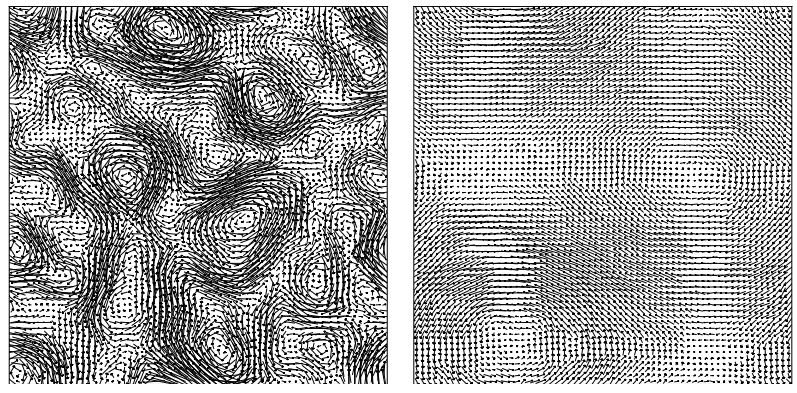
\includegraphics[scale=0.7]{Figures/research_papers/adami2012-evolution-vel-field-tgv.png}
	\caption{Velocity vector plot at $t=2$ (left) and $t=30$ (right). $Re = \infty$. Ref: \parencite{Adami2012} }
	\label{fig:adami2012-evolution-vel-field-tgv}
\end{figure}

The time evolution of the velocity field is given in \ref{fig:adami2012-evolution-vel-field-tgv}, where it can be observed that the $2D$ turbulence is characterised by merging and pairing of small vortices. The energy spectra given in \ref{fig:adami2012-energy-spectra-tgv} show that at low wave numbers, both interpolation schemes give the same results, but at high wave numbers, the results differ. The energy spectrum of the standard SPH has a linear slope of magnitude $m = 1$ in a log-log scale equivalent to a purely noisy velocity field. Theoretically, however, $2D$ turbulence has an energy cascade with a slope of $m = -3$ in the inertial range, which is reasonably predicted using mSPH.
\begin{figure}[h!]
	\centering
	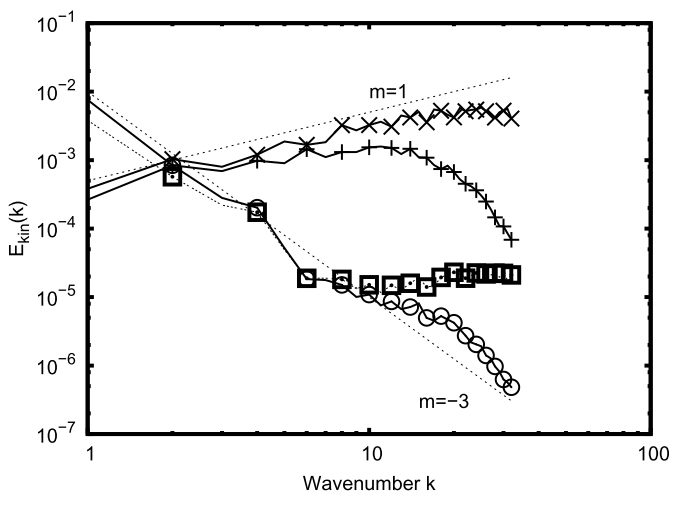
\includegraphics[scale=0.55]{Figures/research_papers/adami2012-energy-spectra-tgv.png}
	\caption{Comparison of energy spectra $t=10$. $+$ and $\times$ denote standard SPH results with quintic spline and MLS interpolation; $\circ$ and $\square$ denote mSPH results with quintic spline and MLS interpolation. Ref: \parencite{Adami2012} }
	\label{fig:adami2012-energy-spectra-tgv}
\end{figure}

The second test case employed by the authors was that of the $3D$ TGV problem requiring $64^3$ particles for a wide range of Reynolds numbers. The dissipation rate of the flow simulations are shown in \ref{fig:adami2012-dissipation-re400} and \ref{fig:adami2012-dissipation-re3000}. It can be observed that the standard SPH is unable to simulate transitional flows due to excessive dissipation. In contrast, mSPH can reproduce the dissipation rate reasonably well. This implies that the corrected particle transport velocity is an analogous eddy-viscosity model on scales below the numerical resolution.
\begin{figure}[h!]
	\centering
	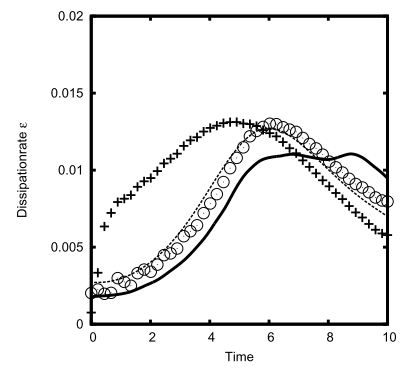
\includegraphics[scale=0.7]{Figures/research_papers/adami2012-dissipation-re400.png}
	\caption{Dissipation rate at $Re = 400$ using DNS (solid line), Smagorinsky model (dashed line), standard SPH ($+$) and mSPH ($\circ$). Ref: \parencite{Adami2012}}
	\label{fig:adami2012-dissipation-re400}
\end{figure}
\begin{figure}[h!]
	\centering
	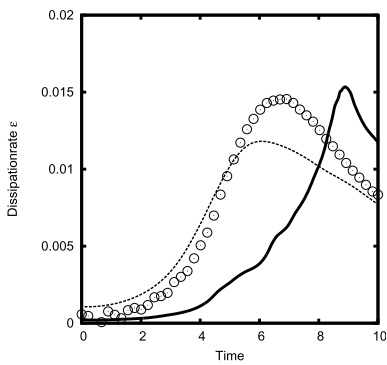
\includegraphics[scale=0.7]{Figures/research_papers/adami2012-dissipation-re3000.png}
	\caption{Dissipation rate at $Re = 3000$ using DNS (solid line), Smagorinsky model (dashed line) and mSPH ($\circ$). Ref: \parencite{Adami2012}}
	\label{fig:adami2012-dissipation-re3000}
\end{figure}

\section{Large Eddy Simulation-based Models}
\subsection{Implicit Pressure Poisson-based Models}
\label{sec:Implicit-Pressure-Poisson-based-Models}
Gotoh et al. \parencite{Gotoh2004} were amongst the first to integrate Large Eddy Simulation techniques with the SPH method. They derived this LES-SPH model, based on incompressible flow, to tackle the problem of reflection and transmission characteristics of regular waves by a partially immersed curtain-type breakwater. In order to compare the dissipation efficiencies, they considered the non-overtopping and overtopping cases of the problem.

The governing equations of the system were described as given by the continuity equation in \ref{eq:Gotoh2004-continuity-governing} and the momentum equation in \ref{eq:Adami2012-mom-governing}.
\begin{equation}
	\frac{1}{\rho} \LagDerivative{\rho} + \nabla \cdot \vect{v} = 0
	\label{eq:Gotoh2004-continuity-governing}
\end{equation}

The LES mass and momentum conservation equations for the flow were derived by filtering the respective equations using a spatial filter $\overline{(...)}$ to obtain their filtered counter-parts as given by \ref{eq:Gotoh2004-continuity-filtered} and \ref{eq:Gotoh2004-mom-filtered} respectively.
\begin{equation}
	\frac{1}{\rho} \LagDerivative{\rho} + \nabla \cdot \vect{\overline{v}} = 0
	\label{eq:Gotoh2004-continuity-filtered}
\end{equation}
\begin{equation}
	\LagDerivative{\vect{\overline{v}}} = -\frac{1}{\rho}\nabla \overline{P} + \nu \Delta ( \vect{\overline{v}} ) + \frac{1}{\rho}\nabla\cdot\tensor{\tau} + \vect{F}
	\label{eq:Gotoh2004-mom-filtered}
\end{equation}
\begin{equation}
	\frac{1}{\rho} \tensor{\tau} = \vect{\overline{v}} \otimes \vect{\overline{v}} - \overline{\vect{v} \otimes \vect{v}}
	\label{eq:Gotoh2004-stress-tensor}
\end{equation}

The stress tensor defined in \ref{eq:Gotoh2004-stress-tensor} is closed using Boussinesq's Hypothesis as defined in \ref{eq:Gotoh2004-boussinesq}.
\begin{equation}
	\frac{1}{\rho} \tensor{\tau} = 2\nu_t \tensor{S} - \frac{2}{3}k\tensor{I}
	\label{eq:Gotoh2004-boussinesq}
\end{equation}

The turbulent eddy viscosity is estimated using a modified Smagorinsky model as given in \ref{eq:Gotoh2004-eddy-visc}. This allows wall effects to be incorporated into the model, which the authors required to tackle the problem they were working on.
\begin{equation}
	\nu_t = \min(C_s \Delta x, \kappa d_{wall})^2 \sqrt{2 \FrobeniusInnerProduct{S}{S}}
	\label{eq:Gotoh2004-eddy-visc}
\end{equation}
\begin{equation}
	C_s=0.1, \kappa=0.4
\end{equation}

Where $(C_s)$ is the Smagorinsky constant, $(\kappa)$ is the von Karman constant and $d_{wall}$ is the normal distance of the particle to the closest wall.
The first term in \ref{eq:Gotoh2004-eddy-visc} dominates the flow far away from the solid wall, thereby recovering the standard Smagorinsky model. However, the second term dominates for flow close to the wall; hence, the eddy viscosity is a function of the particle distance to the wall. This overcomes the disadvantage of the standard Smagorinsky being over-dissipative inside the laminar layer.

In order to solve the system of equations and evolve them in time, the authors employed the Predictive-Corrective time integrator, similar to the two-step projection method of Chorin \parencite{chorin1968numerical}. The prediction stage is outlined by \ref{eq:Gotoh2004-predict-start} - \ref{eq:Gotoh2004-predict-end}. 
\begin{equation}
	\Delta \vect{v}_* = \bigg( \nu \Delta ( \vect{\overline{v}} ) + \frac{1}{\rho}\nabla\cdot\tensor{\tau} + \vect{F} \bigg) \Delta t
	\label{eq:Gotoh2004-predict-start}
\end{equation}
\begin{equation}
	\vect{v}_* = \vect{v}_t + \Delta \vect{v}_*
\end{equation}
\begin{equation}
	\vect{r}_* = \vect{r}_t + \vect{v}_* \Delta t
	\label{eq:Gotoh2004-predict-end}
\end{equation}

The correction stage is outlined by \ref{eq:Gotoh2004-correct-start} - \ref{eq:Gotoh2004-correct-end}. $(\overline{P})$ which is required to update the $(\vect{v}_{t+1})$ term is calculated implicitly from \ref{eq:Gotoh2004-correct-pressure-implicit}, which is based on the filtered continuity equation given by \ref{eq:Gotoh2004-continuity-filtered} and assuming incompressibility $\LagDerivative{\rho}=0$.
\begin{equation}
	\Delta \vect{v}_{**} = -\frac{1}{\rho} \nabla \overline{P}_{t+1} \Delta t
	\label{eq:Gotoh2004-correct-start}
\end{equation}
\begin{equation}
	\nabla \cdot \bigg( \frac{1}{\rho_*} \nabla \overline{P}_{t+1} \bigg) = \frac{\rho_0 - \rho_*}{\rho_0 \Delta t^2}
	\label{eq:Gotoh2004-correct-pressure-implicit}
\end{equation}
\begin{equation}
	\vect{v}_{t+1} = \vect{v}_* + \Delta \vect{v}_{**}
\end{equation}
\begin{equation}
	\vect{r}_{t+1} = \vect{r}_t + (\vect{v}_t + \vect{v}_{t+1})\frac{\Delta t}{2}
	\label{eq:Gotoh2004-correct-end}
\end{equation}

In order to solve the system of equations given by \ref{eq:Gotoh2004-predict-start} - \ref{eq:Gotoh2004-correct-end} in an SPH setting, the authors presented the following SPH formulation for the flow property. \textit{Note:} The over-line $\overline{(...)}$ convention used to denote filtered flow properties will be dropped in this sub-section unless stated otherwise.

The fluid density is given using a simple summation density \ref{eq:Gotoh2004-summation-density}.
\begin{equation}
	\rho_i = \sum_j m_j\WIJ
	\label{eq:Gotoh2004-summation-density}
\end{equation}

The pressure gradient term is defined in \ref{eq:Gotoh2004-grad-p-sph} in a symmetric form.
\begin{equation}
	\bigg( \frac{1}{\rho} \nabla P \bigg)_i = \sum_j m_j \bigg( \frac{P_i}{\rho_i^2} + \frac{P_j}{\rho_j^2} \bigg) \DWIJ
	\label{eq:Gotoh2004-grad-p-sph}
\end{equation}

The divergence of $\vect{v}$ is also defined symmetrically as given by \ref{eq:Gotoh2004-div-u-sph}.
\begin{equation}
	\nabla \cdot \vect{v}_i = \rho_i \sum_j m_j \bigg(\frac{\vect{v}_i}{\rho^2_i} + \frac{\vect{v}_j}{\rho^2_j} \bigg) \cdot \DWIJ
	\label{eq:Gotoh2004-div-u-sph}
\end{equation}

The pressure Laplacian, defined in \ref{eq:Gotoh2004-p-laplacian-sph}, is formulated as a hybrid of a standard SPH first derivative with a finite difference approximation for the first derivative to aid particle pressure stability \parencite{cummins1999sph}.
\begin{equation}
	\nabla \cdot \bigg( \frac{1}{\rho} \nabla P \bigg)_i = \sum_j m_j \frac{8}{(\rho_i + \rho_j)^2} \frac{P_{ij} \RIJ \cdot \DWIJ }{\RtwoIJ}
	\label{eq:Gotoh2004-p-laplacian-sph}
\end{equation}

The divergence of the stress tensor is defined in \ref{eq:Gotoh2004-div-tau-sph}.
\begin{equation}
	\bigg( \frac{1}{\rho} \nabla \cdot \tensor{\tau} \bigg)_i = \sum_j m_j \Bigg( \frac{1}{\rho_i^2}\tensor{\tau_i} + \frac{1}{\rho_j^2}\tensor{\tau_j} \Bigg) \cdot \DWIJ
	\label{eq:Gotoh2004-div-tau-sph}
\end{equation}

Finally, the laminar stress term, consisting of the velocity Laplacian term, is defined as given by \ref{eq:Gotoh2004-vel-laplacian-sph}.
\begin{equation}
	\big(\nu \Delta(\vect{v}) \big)_i = \sum_j m_j \frac{4(\eta_i + \eta_j)}{(\rho_i + \rho_j)^2}\frac{\VIJ \RIJ \cdot \DWIJ}{\RtwoIJ}
	\label{eq:Gotoh2004-vel-laplacian-sph}
\end{equation}

The authors used this SPH-LES model to investigate the wave interaction with a partially immersed breakwater and compared the results with experimentally obtained values of a similar setup. Their computational domain was $2D$ populated by $\approx 12e3$ particles.

\begin{figure}[h!]
	\centering
	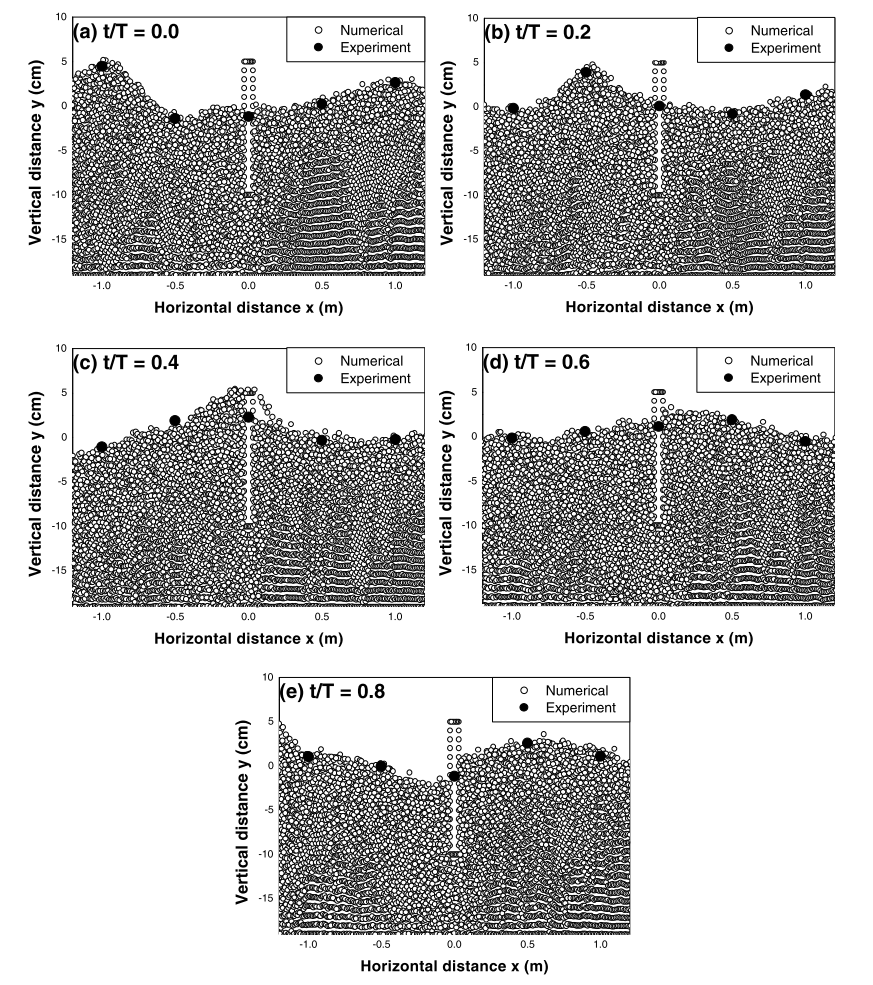
\includegraphics[scale=0.8]{Figures/research_papers/gotoh2004-wave-profile-result.png}
	\caption{Time sequences of computational and experimental wave profiles near curtain wall (overtopping). Ref: \parencite{Gotoh2004}}
	\label{fig:gotoh2004-wave-profile-result}
\end{figure}

As observed in the comparative plots given in \ref{fig:gotoh2004-wave-profile-result}, the model proves to be accurate in tracking free surfaces of large deformation without numerical diffusion. The authors also observed the model's capability to simulate turbulence and eddy vortices realistically near the curtain wall. However, the authors also conclude that a more refined turbulence model will be required for further accuracy in predicting flow involving wave interactions.

Building on the work mentioned above, Shao and Gotoh \parencite{Shao2005} performed a comparative study of SPH and the Moving Particle Semi-Implicit (MPS) method coupled with an LES model. They also validated these models against experimental data.

The filtered conservation equations which the authors considered were the same as given by \ref{eq:Gotoh2004-continuity-filtered} - \ref{eq:Gotoh2004-boussinesq}. However, they incorporated the standard Smagorinsky model \parencite{smagorinsky1963general} given by \ref{eq:Shao2005-eddy-visc} as opposed to the modified model \ref{eq:Gotoh2004-eddy-visc}.
\begin{equation}
	\nu_t = (C_s \Delta x)^2
	\label{eq:Shao2005-eddy-visc}
\end{equation}

The authors consider the same predictive-corrective scheme to evolve their system as detailed in \ref{eq:Gotoh2004-predict-start} - \ref{eq:Gotoh2004-correct-end}.
Similarly, they follow the same SPH formulation outlined in \ref{eq:Gotoh2004-summation-density} - \ref{eq:Gotoh2004-vel-laplacian-sph}. They do however, slightly modify the pressure and velocity Laplacian terms as given in \ref{eq:Shao2005-P-laplacian-sph} and \ref{eq:Shao2005-vel-laplacian-sph} respectively.
\begin{equation}
	(\nabla^2 P)_i = \sum_j m_j \frac{4}{\rho_i + \rho_j} \frac{P_{ij} \RIJ \cdot \DWIJ }{\RtwoIJ}
	\label{eq:Shao2005-P-laplacian-sph}
\end{equation}
\begin{equation}
	\big(\nu \Delta(\vect{v}) \big)_i = \sum_j m_j \frac{2(\nu_i + \nu_j)}{\rho_i + \rho_j}\frac{\VIJ \RIJ \cdot \DWIJ}{\RtwoIJ}
	\label{eq:Shao2005-vel-laplacian-sph}
\end{equation}

The authors validated this SPH-LES Model using experimental data from the experimental data corresponding to a solitary wave breaking on the beach \parencite{Synolakis1986}. Their computational domain was $2D$ and consisted of $\approx 18e3$ particles. 
From the computed wave profiles shown in \ref{fig:shao2005-wave-profile-result}, it can be visually observed that there is reasonable agreement between the experimental and computation data. This verifies the model's accuracy in tracking free surfaces with less or no numerical diffusion.
Furthermore, by performing a convergence study of the SPH-LES model using the dam-break problem, the authors could show that the scheme's spatial and temporal accuracy is $O(\Delta t + \Delta x^(1.25)$.

\begin{figure}[h!]
	\centering
	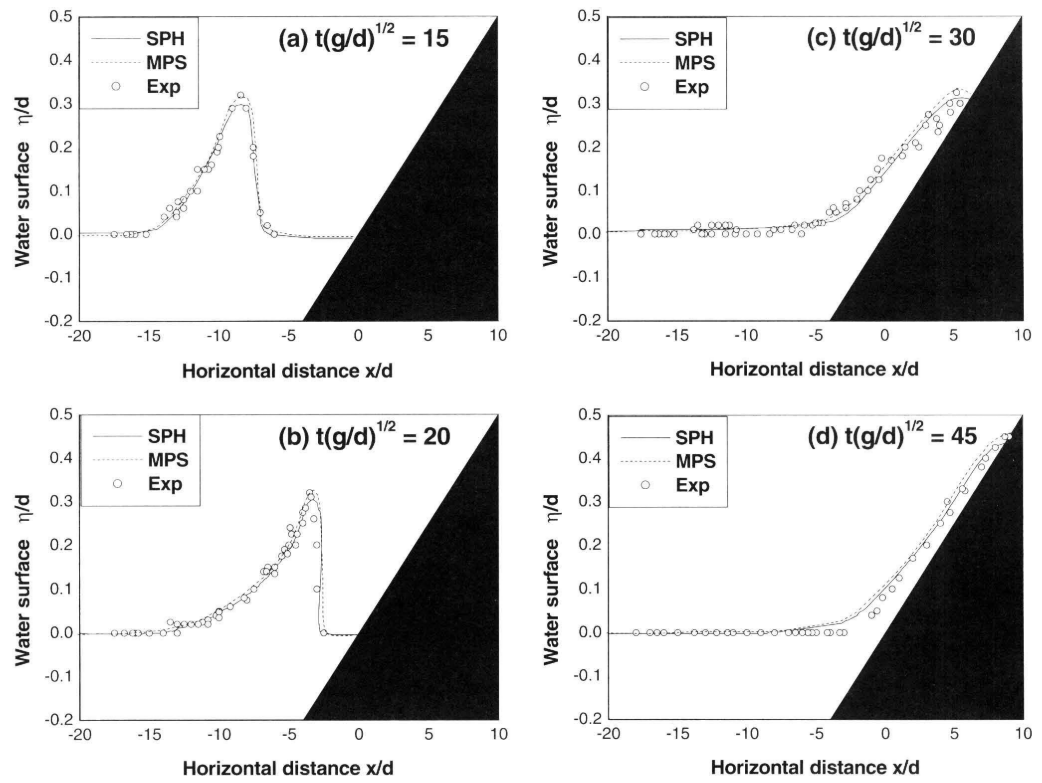
\includegraphics[scale=0.6]{Figures/research_papers/shao2005-wave-profile-result.png}
	\caption{Experimental and computational wave profiles by SPH and MPS model. Ref: \parencite{Shao2005}}
	\label{fig:shao2005-wave-profile-result}
\end{figure}


\subsection{Explicit Pressure Equation of State-based Solvers}
\subsubsection{Standard Smagorinsky Model}

Rogers and Dalrymple \parencite{ROGERS2005}, similar to the work on SPH-LES modelling detailed in \ref{sec:Implicit-Pressure-Poisson-based-Models}, came up with an LES-type sub-particle-scale (SPS) formulation based on the weakly compressible assumption in order to develop a turbulence model for SPH.

The authors considered the mass and momentum conservation equations as already given in \ref{eq:Gotoh2004-continuity-governing} and  \ref{eq:Adami2012-mom-governing} respectively, along with the equation of state \ref{eq:violeau-eos}. However, for the value of $(B)$ in the state equation, the authors considered the definition given in \ref{eq:ROGERS2005-eos-b}:
\begin{equation}
	B = 10 u_{max}
	\label{eq:ROGERS2005-eos-b}
\end{equation}

They subsequently filtered the compressible conservation equations using Favre averaging as given by \ref{eq:ROGERS2005-favre-averaging}.
\begin{equation}
	\widetilde{f} = \frac{\overline{\rho f}}{\overline{\rho}}
	\label{eq:ROGERS2005-favre-averaging}
\end{equation}

The derived filtered conservation equations for mass and momentum are detailed in \ref{eq:ROGERS2005-continuity-filtered} and \ref{eq:ROGERS2005-mom-filtered}.
\begin{equation}
	\LagDerivative{\overline{\rho}} = -\overline{\rho} \nabla \cdot \vect{\widetilde{v}}
	\label{eq:ROGERS2005-continuity-filtered}
\end{equation}
\begin{equation}
	\LagDerivative{\vect{\widetilde{v}}} = - \frac{1}{\overline{\rho}}\nabla \overline{P} + \frac{1}{\overline{\rho}} (\nabla \cdot \overline{\rho \nu} \nabla) \vect{\widetilde{v}} + \frac{1}{\overline{\rho}}\nabla\cdot\tensor{\tau} + \vect{F}
	\label{eq:ROGERS2005-mom-filtered}
\end{equation}

Where the SPS stress tensor and turbulent eddy viscosity is given by \ref{eq:ROGERS2005-tau} and \ref{eq:ROGERS2005-turbulent-eddy-visc} respectively.
\begin{equation}
	\tensor{\tau} = \overline{\rho}\bigg(2\nu_t \tensor{S} - \frac{2}{3}\operatorname{tr}[\tensor{S}]\tensor{I}\bigg) - \frac{2}{3}\overline{\rho}C_I \overline{\Delta}^2 \tensor{I}, C_I = 6.6e-4
	\label{eq:ROGERS2005-tau}
\end{equation}
\begin{equation}
	\nu_t = (C_s \Delta x)^2 \sqrt{2 \FrobeniusInnerProduct{S}{S}}, C_s = 0.12
	\label{eq:ROGERS2005-turbulent-eddy-visc}
\end{equation}

As for the SPH formulations of the aforementioned governing equations, the authors

The authors derived the SPH formulations of the aforementioned governing equations. The continuity equation takes the form as detailed in \ref{eq:violeau-continuity}. The pressure gradient term is given in \ref{eq:Gotoh2004-grad-p-sph}. The laminar stress term, consisting of the velocity Laplacian is given by \ref{eq:ROGERS2005-vel-laplacian-sph}, which itself was built on the work of Morris et al. \parencite{morris1997modeling} as given in \ref{eq:morris1997modeling-vel-laplacian-sph}. Finally the stress divergence is defined by \ref{eq:Gotoh2004-div-tau-sph}.
\begin{equation}
	\bigg( \frac{1}{\rho} (\nabla \cdot \eta \nabla) \vect{v} \bigg)_i = \sum_j m_j \frac{\nu (\rho_i + \rho_i)}{\rho_{ij}^2} \frac{\VIJ \RIJ \cdot \DWIJ}{\RtwoIJ + \MachineEpsilon}
	\label{eq:ROGERS2005-vel-laplacian-sph}
\end{equation}
\begin{equation}
	\bigg( \frac{1}{\rho} (\nabla \cdot \eta \nabla) \vect{v} \bigg)_i = \sum_j m_j \frac{(\eta_i + \eta_j) \VIJ}{\rho_i \rho_j} \bigg( \frac{1}{\RtwoIJ[]} \PartialDerivative[r_i]{\WIJ} \bigg), \DWIJ = \frac{\RIJ}{\RtwoIJ[]} \PartialDerivative[r_i]{\WIJ}
	\label{eq:morris1997modeling-vel-laplacian-sph}
\end{equation}

The authors noted that the LES description of viscous effects in
slightly compressible SPH could lead to unphysical behaviour at free surfaces due to density variations being magnified by the equation of state. The lack of artificial viscosity implies that such variations are not damped. They subsequently noted that averaging the density would ensure smooth and physically acceptable free surfaces, based on the work of Panizzo \parencite{panizzo2004physical}. Hence, they performed Shepard filtering of the density as defined in \ref{eq:ROGERS2005-rho-shepard-filter} every 40-time steps.
\begin{equation}
	\rho_i = \frac{\sum_j \rho_j \WIJ \Vol_j}{\sum_j \WIJ \Vol_j}
	\label{eq:ROGERS2005-rho-shepard-filter}
\end{equation}

The authors simulated the problem of a weakly plunging breaker in $2D$ and $3D$ to ascertain the performance and capability of the model. Their $2D$ computational domain consisted of $\approx 1e5$ particles, with the $3D$ domain consisting $\approx 2e4$ particles.
The authors could show that in the case of the $2D$ problem, the model could predict regions of high vorticity that persisted longer when compared to standard SPH utilising conventional artificial viscosity. The model also displayed the turbulent bore, which generated reverse breaking, leading to the downbursting-like phenomenon, as observed in experiments \parencite{kubo2001large}.
In the case of the $3D$ problem, the authors showed the model's capability to capture near vertically-oriented eddies despite the lower resolution. 

Building on this work, Dalrymple and Rogers \parencite{Dalrymple2006} used this scheme on a wide variety of problems, ranging from $2D$ Green water overtopping, $2D$ waves on a beach, $3D$ dam break and $3D$ waves on a beach. The quantitative analysis of the results allowed the authors to conclude that the model is especially suited for problems involving splash or flow separation. The authors also warn about the model's requirement of a large number of particles for sufficient resolution. That and the finite speed of sound stemming from the compressible flow implied that time steps had to $O(10^{-5}s)$. Hence, the authors remain cautiously optimistic about the model since the method performs well for smaller regions where the number of particles is reasonable. However, they believe that extended Boussinesq codes would more efficiently model larger domains.

\subsubsection{Modified Smagorinsky Model}
Canelas et al. \parencite{Canelas2016} constructed the wall-adapting local eddy viscosity (WALE) model to be incorporated in the SPH-LES scheme. They noted that studying turbulent flow fields required the identification of vortices themselves to study their interactions in the flow. They used the definition of Lagrangian Coherent Structures (LCS) to help capture these vortices. As a Lagrangian method, SPH is preferable for studying LCS since the technique provides the motion of individual fluid particles, thereby eliminating the need for expensive post-processing inherent to Eulerian solutions. 
However, they noted that typically employed SPS strategies for LES simulations, based on the standard Smagorinsky model, cannot correctly enforce wall conditions and non-vanishing stresses with laminar flows. Hence they devised the WALE model.

The authors consider the compressible Navier-Stokes (NS) along the continuity equation as their governing equation. They subsequently present the SPH formulation of the continuity equation as defined by \ref{eq:Canelas2016-continuity-sph}.
\begin{equation}
	\LagDerivative{\rho_i} = - \rho_i \sum_j m_j \VIJ \cdot \DWIJ
	\label{eq:Canelas2016-continuity-sph}
\end{equation}
The pressure gradient term is given in \ref{eq:Gotoh2004-grad-p-sph}. The laminar stress term, consisting of the velocity Laplacian, is given by \ref{eq:Canelas2016-vel-laplacian-sph}. 
\begin{equation}
	\big(\nu \Delta(\vect{v}) \big)_i = \sum_j m_j \frac{4 \nu}{\rho_i + \rho_j}\frac{\VIJ \RIJ \cdot \DWIJ}{\RtwoIJ}
	\label{eq:Canelas2016-vel-laplacian-sph}
\end{equation}

Finally the stress divergence is defined by \ref{eq:Gotoh2004-div-tau-sph}, with the stress tensor being defined by \ref{eq:Canelas2016-tau}
\begin{equation}
	\tensor{\tau} = \rho \bigg( 2\nu_t \tensor{S} - \frac{2 \nu_t}{3}\operatorname{tr}[\tensor{S}]\tensor{I} \bigg) - \frac{4}{3} \rho C_I \Delta^2 \tensor{I} \FrobeniusInnerProduct{S}{S}, C_I = 6.6e-3
	\label{eq:Canelas2016-tau}
\end{equation}

The WALE model redefines the turbulent eddy viscosity as given by \ref{eq:Canelas2016-turbulent-eddy-visc}.
\begin{equation}
	\nu_t = \rho (C_w \Delta x)^2 \frac{\FrobeniusInnerProduct{S^d}{S^d}^{3/2}}{\FrobeniusInnerProduct{S}{S}^{5/2} + \FrobeniusInnerProduct{S^d}{S^d}^{5/4}}, C_w=0.325
	\label{eq:Canelas2016-turbulent-eddy-visc}
\end{equation}
Where
\begin{equation}
	\tensor{S^d} = \HalfFrac \bigg( (\nabla \vect{v})^2 + \big((\nabla \vect{v})^T\big)^2 \bigg) - \frac{1}{3} \operatorname{tr}[(\nabla \vect{v})^2] \tensor{I}
\end{equation}

In order to test their model, the authors considered an array of cylinders in fluid flow as shown in \ref{fig:Canelas2016-vel-field}, with a constant body force. They computed the vorticity field and the Finite-Time Lyapunov Exponents (FTLE) field to study the LCSs in the flow. These fields are shown in \ref{fig:Canelas2016-vorticity-field} and \ref{fig:Canelas2016-ftle-field} respectively.
\begin{figure}[h!]
	\centering
	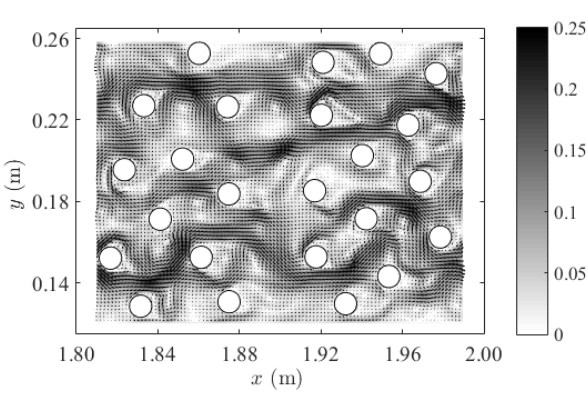
\includegraphics{Figures/research_papers/Canelas2016-vel-field.png}
	\caption{Cylinder distribution and instantaneous velocity overlapped by velocity vectors. Velocity in $m/s$, at $t=20s$. The flow direction is from left to right. Ref: \parencite{Canelas2016}}
	\label{fig:Canelas2016-vel-field}
\end{figure}
\begin{figure}[h!]
	\centering
	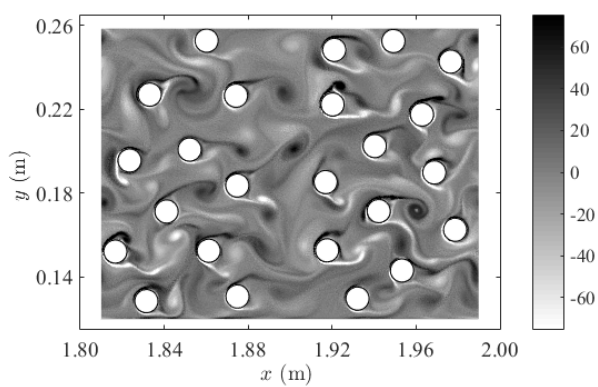
\includegraphics{Figures/research_papers/Canelas2016-vorticity-field.png}
	\caption{Vorticity field. Vorticity in Hz, at $t = 20s$. Ref: \parencite{Canelas2016}}
	\label{fig:Canelas2016-vorticity-field}
\end{figure}
\begin{figure}[h!]
	\centering
	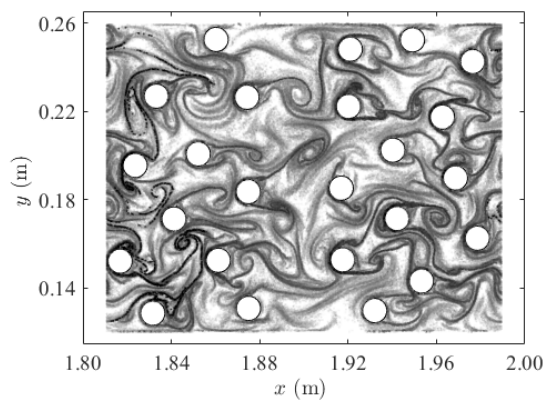
\includegraphics{Figures/research_papers/Canelas2016-ftle-field.png}
	\caption{FTLE field with negative integration time $(T = -0.4 s)$ (unstable manifolds - attracting LCS) at $t = 20s$. Ref: \parencite{Canelas2016}}
	\label{fig:Canelas2016-ftle-field}
\end{figure}

\subsection{Quasi-Lagrangian Models}

\subsection{RANS-based $k-\epsilon$ Models}

Shao \parencite{Shao2006} demonstrated that the two-equation $k-\epsilon$ model, an extensively studied model derived from the Reynolds-averaged Navier–Stokes (RANS) equations, can be incorporated in the truly incompressible version of SPH (ISPH). By attempting to extend RANS equations, which are hugely successful in practical fields, to a mesh-free method such as SPH, the author provides a framework to build on the wide variety of closure models available.

To discretise the RANS equations to an SPH form, the author considers the Reynolds averaged mass and momentum conservation equations as given in \ref{eq:Shao2006-rans-continuity-governing} and \ref{eq:Shao2006-rans-mom-governing} respectively. \textit{Note:} The averaged flow properties are represented without any over-line $\overline{(...)}$ hereafter.
\begin{equation}
	\frac{1}{\rho} \LagDerivative{\rho} + \nabla \cdot \vect{v} = 0, \LagDerivative{\rho} = 0 \text{ (Incompressible)}
	\label{eq:Shao2006-rans-continuity-governing}
\end{equation}
\begin{equation}
	\LagDerivative{\vect{v}} = -\frac{1}{\rho}\nabla P + \nu \Delta( \vect{v} ) + \frac{1}{\rho} \nabla \cdot \tensor{\tau} + \vect{F}
	\label{eq:Shao2006-rans-mom-governing}
\end{equation}

The stress tensor is given by \ref{eq:Gotoh2004-boussinesq}, while the turbulent eddy viscosity is defined as \ref{eq:Shao2006-turbulent-eddy-visc}.
\begin{equation}
	\nu_t = c_d \frac{k^2}{\epsilon}
	\label{eq:Shao2006-turbulent-eddy-visc}
\end{equation}

The transport equations for the turbulent kinetic energy and dissipation rate is given by \ref{eq:Shao2006-k-transport-eq} and \ref{eq:Shao2006-eps-transport-eq} respectively.
\begin{equation}
	\LagDerivative{k} = \nabla \cdot \bigg( \frac{\nu_t}{\sigma_k} \nabla k \bigg) + P_k - \epsilon
	\label{eq:Shao2006-k-transport-eq}
\end{equation}
\begin{equation}
	\LagDerivative{\epsilon} = \nabla \cdot \bigg( \frac{\nu_t}{\sigma_{\epsilon}} \nabla \epsilon \bigg) + c_{1\epsilon} \frac{\epsilon}{k} P_k - c_{2\epsilon} \frac{\epsilon^2}{k}
	\label{eq:Shao2006-eps-transport-eq}
\end{equation}
\begin{equation}
	P_k = 2\nu_t \FrobeniusInnerProduct{S}{S}
	\label{eq:Shao2006-k-production-term}
\end{equation}

Where, $(\sigma_k, \sigma_{\epsilon}, c_{1\epsilon}, c_{2\epsilon}) = (1.0, 1.3, 1.44, 1.92)$ are empirical constants dependent on the nature of the flow , and $(P_k)$ is the turbulence production rate, which satisfies the relation given by \ref{eq:pope2000turbulent-k-production-relation} \parencite{pope2000turbulent}.
\begin{equation}
	\frac{P_k}{\epsilon} = c_d \Bigg( \frac{\sqrt{2 \FrobeniusInnerProduct{S}{S}}}{\epsilon} \Bigg)
	\label{eq:pope2000turbulent-k-production-relation}
\end{equation}

These governing equations are solved and evolved using the same predictive-corrective time integrator as seen in the work of \parencite{Gotoh2004}, and outlined in \ref{eq:Gotoh2004-predict-start} - \ref{eq:Gotoh2004-correct-end}.

As for the SPH formulations of the governing equations, the author builds on the work of \parencite{Gotoh2004}, and uses the same discretization as defined in \ref{eq:Gotoh2004-summation-density} - \ref{eq:Gotoh2004-div-tau-sph}. However, the author uses a slightly modified version of the laminar stress term given in \ref{eq:Gotoh2004-vel-laplacian-sph} and redefines it as given in \ref{eq:Shao2006-vel-laplacian-sph}.
\begin{equation}
	\big(\nu \Delta(\vect{v}) \big)_i = \sum_j m_j \frac{2 ( \nu_i + \nu_j ) }{ \rho_i + \rho_j }\frac{\VIJ \RIJ \cdot \DWIJ}{\RtwoIJ}
	\label{eq:Shao2006-vel-laplacian-sph}
\end{equation}

The author tested the model on the problem of $2D$ wave breaking and overtopping of a sloping wall and compared the results obtained against experimental data \parencite{li2004wave} to validate the model—the computational domain of $\approx 6e3$ particles.

As seen from the evolution of the water surface elevation plotted in \ref{fig:Shao2006-water-surf-elevations}, the author could ascertain that the proposed model produced better results than those of Li et al. \parencite{li2004wave}, compared to the experimental data in \ref{fig:Shao2006-water-surf-elevations}(a) and \ref{fig:Shao2006-water-surf-elevations}(b). This could be attributed to the free surfaces being accurately tracked by particles without numerical diffusion. 
In \ref{fig:Shao2006-water-surf-elevations}(c) and \ref{fig:Shao2006-water-surf-elevations}(d), despite the wave profiles being consistent with each other in phase and shape, the proposed model predicts smaller elevation levels. Li et al. use a dynamic Smagorinsky model, whereas the proposed model uses constant empirical coefficients. The author believes these coefficients derived from a quasi-steady state may behave sub-optimally in transient flow, such as the problem at hand.
\begin{figure}[h!]
	\centering
	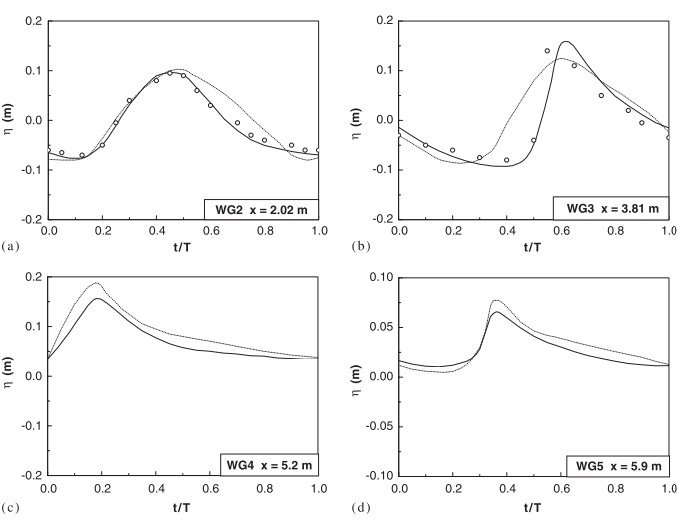
\includegraphics[scale=0.9]{Figures/research_papers/Shao2006-water-surf-elevations.png}
	\caption{Comparisons of computed water surface elevations by SPH (solid lines) with experimental ($\circ$) and numerical (dotted lines) data of Li et al. \parencite{li2004wave}. Ref: \parencite{Shao2006}}
	\label{fig:Shao2006-water-surf-elevations}
\end{figure}

The author concludes that the $k-\epsilon$ model would require further sensitivity analysis for the turbulence model and spatial resolution for improved results, despite being reasonably accurate in tracking free surfaces.

Wang and Liu \parencite{Wang2020} build on the work of Shao \parencite{Shao2006} to further improve the ISPH $k-\epsilon$ model. They achieved this by using the modelling and computational developments which SPH has benefited from since the work of Shao.
The authors here consider the same SPH discretised equations and two-step time integrator as Shao, with two distinct modifications in the Pressure Poisson equation as given by \ref{eq:Wang2020-correct-pressure-implicit} instead of \ref{eq:Gotoh2004-correct-pressure-implicit}. They also redefined propagation equation for $(\vect{r}$ using \ref{eq:Wang2020-correct-end} instead of \ref{eq:Gotoh2004-correct-end}.
\begin{equation}
	\nabla \cdot \bigg( \frac{1}{\rho_0} \nabla P_{t+1} \bigg) = \frac{1}{\Delta t} \nabla \cdot \vect{u_*}
	\label{eq:Wang2020-correct-pressure-implicit}
\end{equation}
\begin{equation}
	\vect{r}_{t+1} = \vect{r}_* + \Delta \vect{v}_{**} \Delta t
	\label{eq:Wang2020-correct-end}
\end{equation}

The authors also provided SPH discretization for the transport equations for $(k)$ and $(\epsilon)$ using \ref{eq:Wang2020-k-laplacian} and \ref{eq:Wang2020-eps-laplacian} which requires the use of particle density $(\varphi)$ as given in \ref{eq:Wang2020-particle-density}.
\begin{equation}
	\varphi_i = \sum_j \WIJ
	\label{eq:Wang2020-particle-density}
\end{equation}
\begin{equation}
	\nabla \cdot \bigg( \frac{\nu_t}{\sigma_k} \nabla k \bigg)_i = - \sum_j \frac{1}{\varphi_j} \bigg( \frac{\nu_{t,i}}{\sigma_k} + \frac{\nu_{t,i}}{\sigma_k}  \bigg) \frac{k_{ij} \RIJ \DWIJ}{\RtwoIJ}
	\label{eq:Wang2020-k-laplacian}
\end{equation}
\begin{equation}
	\nabla \cdot \bigg( \frac{\nu_t}{\sigma_{\epsilon}} \nabla \epsilon \bigg)_i = - \sum_j \frac{1}{\varphi_j} \bigg( \frac{\nu_{t,i}}{\sigma_{\epsilon}} + \frac{\nu_{t,i}}{\sigma_{\epsilon}}  \bigg) \frac{\epsilon_{ij} \RIJ \DWIJ}{\RtwoIJ}
	\label{eq:Wang2020-eps-laplacian}
\end{equation}

The authors also derived an SPH formulation for the strain rate tensor defined in \ref{eq:Wang2020-strain-rate-tensor}, which is based on the studies done on kernel correction \parencite{bonet1999variational, khayyer2008corrected} and given by \ref{eq:Wang2020-vel-grad-term} and \ref{eq:Wang2020-corrective-matrix}. 
\begin{equation}
	\tensor{S}_i = \HalfFrac \bigg( \nabla \vect{v}_i + (\nabla \vect{v}_i)^T \bigg)
	\label{eq:Wang2020-strain-rate-tensor}
\end{equation}
\begin{equation}
	\nabla \vect{v}_i = - \sum_j \frac{1}{\varphi_j} \VIJ \otimes \tensor{L}_i \DWIJ
	\label{eq:Wang2020-vel-grad-term}
\end{equation}
\begin{equation}
	\tensor{L}_i = \Bigg(- \sum_j \frac{1}{\varphi_j} \DWIJ \otimes \RIJ \Bigg)^{-1}
	\label{eq:Wang2020-corrective-matrix}
\end{equation}

The authors validated the model against the problem of a solitary wave propagating over a bottom-mounted barrier in $2D$. Its results are shown in \ref{fig:Wang2020-wave-propogation-result}. They also considered the problem involving wave breaking on a slopping wall in $2D$, which is shown in \ref{fig:Wang2020-wave-breaking-result}.
\begin{figure}[h!]
	\centering
	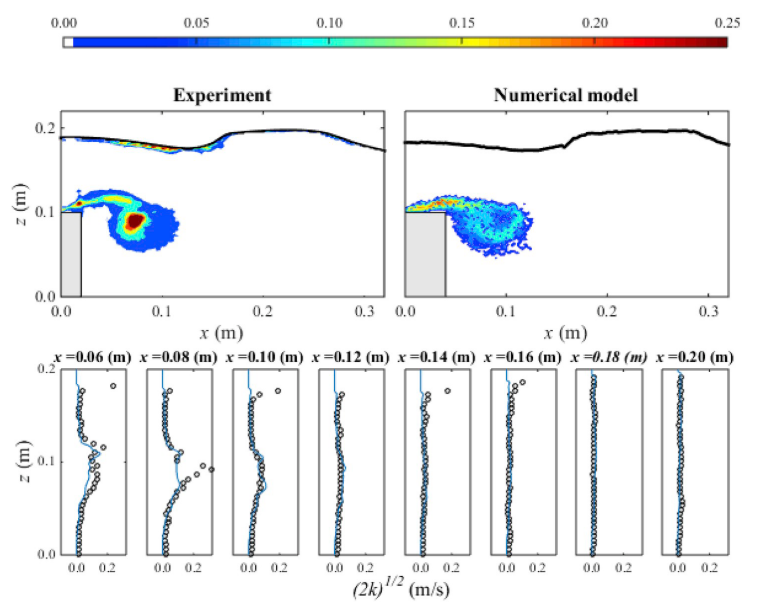
\includegraphics[scale=0.75]{Figures/research_papers/Wang2020-wave-propogation-result.png}
	\caption{Comparisons between experimental data (left) and numerical results (right) for turbulence intensity $(m/s)$ at $t=0.6s$ (top panels) and the corresponding vertical cross-sections (lower panels). In the lower panels, solid lines and $\circ$ represent the numerical and experimental results, respectively. Ref: \parencite{Wang2020}}
	\label{fig:Wang2020-wave-propogation-result}
\end{figure}
\begin{figure}[h!]
	\centering
	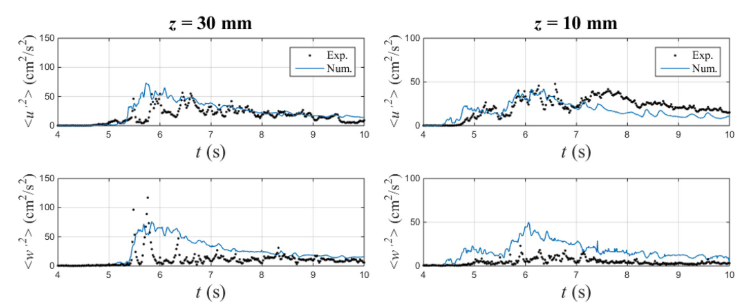
\includegraphics[scale=0.8]{Figures/research_papers/Wang2020-wave-breaking-result.png}
	\caption{Comparisons of numerical and experimental turbulent kinetic energy in x-direction and y-direction. Ref: \parencite{Wang2020}}
	\label{fig:Wang2020-wave-breaking-result}
\end{figure}

Given the model's accuracy, as observed from the figures, the authors conclude that the model's capabilities have been demonstrated, especially in tracking transient-free surfaces. They also reproduce the evolution of turbulence and its intensity due to flow separation. 
However, they note that the model under-predicts the max turbulent kinetic energy and is sensitive to the initial seeding of the turbulent kinetic energy property.
The authors also state that the counteracting effects of the physical viscous dissipation and numerical dissipation, dependent on the particle resolution, would have to be appropriately balanced.
Finally, the authors conclude on the importance of boundary treatment and the need for more sophisticated boundary models to extend the model to $3D$ domains.

%TODO: Need to include Wang2022.

\subsection{LANS-based Models}
So far, having dealt with RANS and LES models of turbulence, a few fundamental drawbacks of these techniques have been brought to light.
In the case of RANS, the flow field is decomposed into
an averaged mean flow and a fluctuating field. Such a decomposition of the NS equations provides differential equations for the mean flow containing contributions from the time-varying turbulent motion. Therefore a closure model is required to capture the effects of the fluctuations on the mean flow. However, by studying only the mean flow quantities, the complete nature of the flow, notwithstanding the complex structures stemming from these fluctuations, cannot be studied, let alone appreciated.

On the face of it, LES would have made for a reasonable alternative to model turbulent flows. This is because the large scales in the flow are resolved by the standard NS equations, while the effects of smaller scales are modelled. However, this remains easier said than done since inhomogeneous and wall-bounded flows necessitate the LES filter width to vary dynamically to capture the average size of turbulent eddies.

The other widespread method of tackling turbulence involves Direct Numerical Simulation (DNS). However, because of the exponentially increasing degrees of freedom as the Reynolds number increases, this technique effectively places an inviolable upper bound on the $Re$ for a given simulation because of computational limitations.

In order to tackle the issues above and address them reasonably, we look for possible solutions. One such solution is the Lagrangian averaging method introduced by Holm et al. \parencite{holm1998euler} and Marsden and Shkoller \parencite{Marsden2001}. In this method, unlike the averaging or filtering of the NS equations as done in RANS or LES, the Lagrangian averaging approach averages at the level of the variational principle from which the Navier–Stokes equations are derived. This procedure yields the Lagrangian-averaged Navier Stokes-$\alpha$ (LANS-$\alpha$) equations, which describe the time evolution of large eddies in turbulent flows. It can be stated that this approach is similar to that of LES.

The LANS-$\alpha$ equations, assuming incompressibility and isotropic turbulence, are derived and simplified by Mohseni et al. \parencite{Mohseni2003}. These equations are as follows:
\begin{equation}
	\nabla \cdot \vect{v} = 0
\end{equation}
\begin{equation}
	\LagDerivative{\vect{v}} = \tensor{\sigma}(\vect{v})
\end{equation}
\begin{equation}
	\tensor{\sigma}(\vect{v}) = -P\tensor{I} + 2\nu(1 - \alpha^2\Delta)\tensor{S} + 2\alpha^2\Dot{\tensor{S}}
\end{equation}
\begin{equation}
	\Dot{\tensor{S}} = \LagDerivative{\tensor{S}} + \tensor{S}\tensor{R} - \tensor{R}\tensor{S}
\end{equation}
\begin{equation}
	\tensor{R} = \HalfFrac\bigg(\nabla\vect{v}-(\nabla\vect{v})^T\bigg)
\end{equation}
Where $\alpha$ denotes the scale of rapid fluctuations in the flow map, wherein, for scales smaller than $\alpha$, the wave activity is filtered by a nonlinear energy redistribution.

Monaghan \parencite{Monaghan2002}, building on the work of Holm \parencite{holm1998euler}, attempted to formulate an SPH version of the continuum LANS-$\alpha$ equations. His work provided one of the earliest models of turbulence in compressible flow. The author incorporated some of his earlier work on XSPH \parencite{monaghan1989problem}, in which particles are moved with a smoothed velocity, leaving the acceleration equation unchanged. The smoothed velocity denoted an average over the velocities of the neighbouring particles. This facilitated the author in writing the Lagrangian analysed by Holm in an SPH form, allowing for the subsequent derivation of the momentum equation, albeit being elaborate and highly complicated. Nevertheless, in conjunction with the continuity equation, the derived momentum equation formulated the SPH-$\alpha$ model, which essentially consisted of an SPH particle moving with the transport velocity smoothed from momentum velocity by an iterative algorithm with an additional dissipation term meant to mimic the standard LES model.

Hu and Adams \parencite{Hu2015} also devised a turbulence model for incompressible flow based on spatial filtering of the NS equations using SPH approximations termed the SPH-$\sigma$ model. The model shares similarities with the LANS-$\alpha$ model and the SPH-$\alpha$ model, differing by the additional stress term in the model and its approach in evaluating the particle transport velocity. The proposed model is also built on the authors' previous work \parencite{hu2007incompressible}, and hence shares similar numerical techniques. The authors also validated the proposed model on $2D$ flow comprising decaying and forced turbulence cases. Their results suggested that the model could simulate incompressible turbulent flow.

Monaghan \parencite{Monaghan2011, Monaghan2017} subsequently improved on the SPH-$\alpha$ model and derived a more amenable variant of the momentum equation. Since, in this case, the model was parameterised around the smoothing parameter $(\varepsilon)$, the turbulence model was termed the SPH-$\varepsilon$ model. The linearly smoothed velocity is given by \ref{eq:Monaghan2017-xsph-vel-smoothing}.
\begin{equation}
	\widehat{\vect{v}}_i = \vect{v}_i - \varepsilon \sum_j \frac{m_j}{M_0} \VIJ K_{h', ij}, \varepsilon \in [0, 1]
	\label{eq:Monaghan2017-xsph-vel-smoothing}
\end{equation}

Where $(K)$ is a smoothing kernel, which can be different from the kernel used in SPH, its corresponding smoothing length being $(h')$. It is noted that the smoothed velocity preserves the shape of the spectrum of the unsmoothed velocity for short-length scales. However, it reduces the magnitude of the unsmoothed velocity by a factor $(1-\varepsilon)$. 

The equation of state is given by \ref{eq:violeau-eos}, and the momentum equation is given by \ref{eq:Monaghan2017-mom-governing}. The momentum equation's third term on the right-hand side is an extra stress term determined by the smoothing. Its overall effect is to redistribute energy without dissipation.
\begin{equation}
	\LagDerivative{\vect{v}_i} = - \sum_j m_j \bigg( \frac{P_i}{\rho_i^2} + \frac{P_j}{\rho_j^2} \bigg) \DWIJ - \sum_j m_j \Pi_{ij} \DWIJ + \frac{\varepsilon}{2} \sum_j \frac{m_j}{M_0} |\VIJ|^2 \DWIJ
	\label{eq:Monaghan2017-mom-governing}
\end{equation}

Where the viscosity term $(\Pi_{ij})$ is given by \ref{eq:Monaghan2017-Pi-visc-term}, in which $(\alpha)$ is a constant.
\begin{equation}
	\Pi_{ij} = - \frac{2 \alpha c_s \VIJ \cdot \RIJ}{(\rho_i + \rho_j) \RtwoIJ}
	\label{eq:Monaghan2017-Pi-visc-term}
\end{equation}

The particles are subsequently transported using \ref{eq:Monaghan2017-r-transport}.
\begin{equation}
	\LagDerivative{\vect{r}_i} = \widehat{\vect{v}}_i
	\label{eq:Monaghan2017-r-transport}
\end{equation}

The author validated the proposed model by simulating $2D$ flow past a cylinder oscillating sinusoidally in both $x$ and $y$ directions.
The author demonstrated the model's capabilities to predict satisfactory results for the velocity correlation functions, energy spectrum and mixing while having particle resolution be half of that required for a DNS with a resolution the Reynolds length. The author concludes that the model's effectiveness for higher Reynolds numbers and other boundary conditions, such as free surfaces, will need to be studied further.
 
\chapter{Turbulence Analysis} % Main chapter title
\label{Chapter3}

Turbulence, as a phenomenon, has been notoriously difficult for a detailed physical analysis. This is further exacerbated by the seemingly endless complex interactions it gives rise to in the flow as long as any form of energy is provided.
Therefore, while modelling turbulence remains one facet of the problem, visualising and analysing the model is another equally challenging task.

As seen in the previous chapter \ref{Chapter2}, numerous Lagrangian turbulent models seem to be tested for only complex surface flows. However, a systematic analysis of isotropic turbulence problems provides greater insight into the energy spectrum and its corresponding cascade across varying length scales. A reasonable model should be able to capture the characteristic hierarchy of scales through which the energy cascade takes place. The dissipation of kinetic energy finally occurs at the scales of the order of Kolmogorov length, where the flow subsequently becomes laminar. In contrast, the injection of energy in turbulent flow generally occurs at much larger scales.

Hence, appropriate test cases must be used when analysing turbulence.

\section{Benchmark Problems}
\subsection{Taylor-Green Vortex Problem}
The Taylor-Green vortex problem is a challenging case to tackle. The flow is periodic, incompressible and consists of decaying vortices.
The $2D$ case of the problem is analytically defined as given by \ref{eq:2d-tgv-vx} - \ref{eq:2d-tgv-p}.
\begin{equation}
    v_x = -U e^{bt} \cos(2\pi x) \sin(2\pi y)
    \label{eq:2d-tgv-vx}
\end{equation}
\begin{equation}
    v_y = U e^{bt} \sin(2\pi x) \cos(2\pi y)
    \label{eq:2d-tgv-vy}
\end{equation}
\begin{equation}
    p = (U e^{bt})^2 \frac{\cos(4\pi x) + \cos(4\pi y)}{4}
    \label{eq:2d-tgv-p}
\end{equation}
\begin{equation}
    b = -\frac{8\pi}{Re}, Re = \frac{UL}{\nu}
\end{equation}
Where $(U, Re, L)$ are flow constants.

The $3D$ case of the problem, defined for a tri-periodic domain with boundary $(\Boundary = [0, 2\pi]^3)$ is initially set-up as given in \ref{eq:3d-tgv-vx} - \ref{eq:3d-tgv-vz}.
\begin{equation}
    v_{x, 0} = \sin(x) \cos(y) \cos(z)
    \label{eq:3d-tgv-vx}
\end{equation}
\begin{equation}
    v_{y, 0} = -\cos(x) \sin(y) \cos(z)
    \label{eq:3d-tgv-vy}
\end{equation}
\begin{equation}
    v_{z, 0} = 0
    \label{eq:3d-tgv-vz}
\end{equation}
The corresponding pressure field obtained from solving the pressure Poisson equation for incompressible flow is given by \ref{eq:3d-tgv-p} \parencite{pereira2021modeling}.
\begin{equation}
    P_{0} = P_o + \frac{\rho_o \nu_o^2}{16} \bigg(2 + \cos(2z) \bigg) \bigg(\cos(2x) + \cos(2y) \bigg)
    \label{eq:3d-tgv-p}
\end{equation}

\subsection{Thin Double-Shear Layer}
The thin double-shear layer is a problem often considered to be too difficult to simulate due to the small scales which are produced. 
The main challenge of the problem, as shown by Brown and Minion \parencite{minion1997performance}, occurs when a numerical method produces spurious structures, especially when the flow is sufficiently under-resolved. 
Drikakis and Smolarkiewicz \parencite{drikakis2001spurious} studied the problem's spurious structure to understand its numerical mechanism. They indicated that the spurious structure's generation depends on the advective scheme's choice. 

The initial conditions for the $2D$ periodic flow is given by \ref{eq:2d-tdsl-vx} - \ref{eq:2d-tdsl-vy}.
\begin{equation}
    v_{x, 0} = \tanh \big(80 \times \min[y-0.25, 0.75-y] \big)
    \label{eq:2d-tdsl-vx}
\end{equation}
\begin{equation}
    v_{y, 0} = \delta \sin \big( 2\pi (x+0.25) \big)
    \label{eq:2d-tdsl-vy}
\end{equation}

\subsection{$3D$ Isotropic Turbulence}
The JHU Turbulence Database Cluster \parencite{li2008public} provide a direct numerical simulation (DNS) data set for isotropic, forced turbulence. The data set consists of the DNS output on $1024^3$ spatial points and $1024$ time samples spanning about one large-scale turnover time.

The entire $1024^4$ space-time history of the incompressible DNS simulation $(Re\approx1460)$ is accessible to users remotely through an interface based on the Web-services model. 
The data from the database contains the three velocity components and the pressure. A uniform non-dimensionalised pressure $(P^* = \frac{P}{\rho U^2} + 1)$ is added to the
database pressure, with Mach number Ma 0.1. 

\subsection{$2D$ Confined \& Driven Turbulence}
Based on the test case employed by Monaghan \parencite{Monaghan2017}, a $2D$ fluid confined to a square solid impenetrable boundary is considered $(\Boundary = [0,1]^2)$. A cylinder of radius $(r=0.7)$ is placed at the centre of the box. The circle is subsequently provided with a Lissajous trajectory to follow given by \ref{eq:2d-cdt-x} - \ref{eq:2d-cdt-y}.
\begin{equation}
    x = 0.5 + 0.25 \sin \bigg( \frac{2\pi t}{5} \bigg)
    \label{eq:2d-cdt-x}
\end{equation}
\begin{equation}
    y = 0.5 + 0.25 \sin \bigg( \frac{4\pi t}{5} \bigg)
    \label{eq:2d-cdt-y}
\end{equation}

\subsection{Free Surface Flows}
As seen in numerous works involving turbulence models in the previous chapter, there does not appear to be any dearth of experimental and numerical research on free-surface flows. Problems ranging from the classic $2D$ and $3D$ dam break to wave propagation, wave breaking, water overtopping, and dyke-flow inspired problems can be simulated. The only caveat involved in such cases includes the resolution requirements of the problem and the approach taken in free surfaces boundary condition implementation.

\section{Post-Simulation Analysis}
\subsection{Energy Spectral Density}
In order to analyse the predicted flow and validate the turbulent model, energy spectra are the most used description since it has to fall off as prescribed by the  Kolmogorov - $5/3$ Law.
Typical mesh or grid-based methods facilitate the calculation of $(E[\WaveNumber])$ by using the Fourier transform of the velocity field as given in \ref{eq:Shi2013-vel-FT}, to obtain the velocity spectrum as defined in \ref{eq:Shi2013-vel-spectrum}.
\begin{equation}
    \vect{V}(\vect{k}) = \frac{1}{L^3} \int i \exp(\vect{k} \cdot \vect{r}) \vect{v}(r\vect{r}) d\vect{r}
    \label{eq:Shi2013-vel-FT}
\end{equation}
Where $(d\vect{r}=dxdy)$ for $2D$ and $(d\vect{r}=dxdydz)$ for $3D$.
\begin{equation}
    E(\vect{k}) = \HalfFrac |\vect{V}(\vect{k}) \cdot \vect{V}^*(\vect{k}) |
    \label{eq:Shi2013-vel-spectrum}
\end{equation}
The energy spectrum is subsequently defined as given by \ref{eq:Shi2013-energy-spectrum} for the case of isotropic turbulence.
\begin{equation}
    E(\WaveNumber) = B \langle E(\vect{k} \rangle, \WaveNumber = |\vect{k}|
    \label{eq:Shi2013-energy-spectrum}
\end{equation}
Where $(B=2\pi k)$ for $2D$ and $(B=4\pi k^2)$ for $3D$.

However, SPH does not have such grid-like data to calculate the energy spectrum directly. Hence, the data has to be reconstructed using interpolation methods as outlined by Shi et al. \parencite{Shi2013}.
The authors provide three distinct methods of interpolating the data across a grid-like space. 
The SPH interpolation method specified by the authors is given in \ref{eq:Shi2013-sph-interpolation}.
\begin{equation}
    A(\vect{r}) \approx \sum_j A_j W(|\vect{r} - \vect{r}_j|, h) \Vol_j
    \label{eq:Shi2013-sph-interpolation}
\end{equation}
The remeshed interpolation method is outlined in \ref{eq:Shi2013-remeshed-interpolation}.
Remeshed Interpolation
\begin{equation}
    A(\vect{r}) \approx \sum_j A_j \Tilde{W}(|x-x_j|, h) \Tilde{W}(|y-y_j|, h) \Tilde{W}(|z-z_j|, h)
    \label{eq:Shi2013-remeshed-interpolation}
\end{equation}
Where $(\Tilde{W})$ represents the kernel where the volume of the particle $(\Vol_j)$ has been absorbed.

The authors also detail the moving least squares (MLS) method as an interpolation tool. Building on the work of Lancaster and Salkauskas \parencite{lancaster1981surfaces}, who were able to extend the $2D$ interpolation technique proposed by Shepard \parencite{shepard1968two} to a general higher-order case. The authors state that they start with a weighted least squares formulation for an arbitrary fixed point and then move said point across the entire domain. This allows for the computation of a weighted least squares fit function, which can be used to evaluate grid-like points.

\subsection{Lagrangian Coherent Structures}
Complex flow cannot only be analysed through primitive flow properties such as pressure, velocity or energy density for a deep understanding of the flow interactions. Techniques using only such properties would fail to identify general coherent structures (CS) in the flow. To facilitate that, quantities such as those employing the velocity gradient, such as the vorticity, Q-criterion, $\Delta$-criterion, swirling strength criterion, etc., are used. 
However, Haller \parencite{haller2005objective} was able to show that in some situations, most of the definitions of the vortex are not objective and suitable for studying the flow, particularly in the context of $3D$ flow.

Therefore, Sun et al. \parencite{sun2016detection} utilise the Lagrangian Coherent Structures (LCSs) as an alternative way with specific advantages for drawing the CSs from a given flow field. In order to identify the LCSs with an objective quantity, the authors use the Finite-time Lyapunov Exponent (FTLE), which represents the rate of separation of the nearby fluid particles over a finite time interval. FTLEs can be evaluated both in forward and backward time directions.

The authors summarise the main advantages of FTLEs over different velocity gradient-based metrics as follows:
\begin{itemize}
    \item Local fluctuations of the velocity field do not induce noise to FTLEs since they are integrated in time.
    
    \item FTLE is formulated in the Lagrangian frameworks allowing for better identification of the LCSs with respect to quantities derived from the velocity gradient.
    
    \item FTLE can identify LCSs with an accuracy that, in some cases, resemble those obtained from advanced experimental techniques.
\end{itemize}

\begin{figure}[h!]
    \centering
    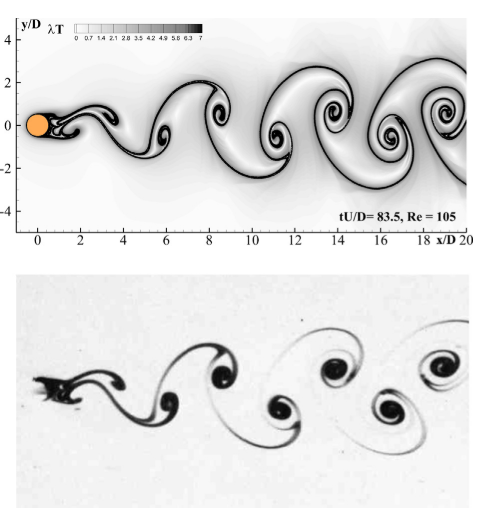
\includegraphics{Figures/research_papers/sun2016detection-fig-1.png}
    \caption{Viscous flow past a circular cylinder at $Re = 105$. Top: Attracting FTLE contour plot from SPH simulation. Bottom: Photo from experiments conducted by Taneda \parencite{taneda1977visual} with electrolytic precipitation in water technique for vortex street visualisation. Ref: \parencite{sun2016detection}}
    \label{fig:sun2016detection-fig-1}
\end{figure}

The forward-in-time FTLE is calculated using the forward-in-time Right-Cauchy–Green strain tensor, while backward-in-time FTLE requires the Left-Cauchy–Green strain tensor.
The authors propose two methods to calculate a flow's Cauchy–Green strain tensors.

The first method uses SPH formulations for the deformation gradient to compute the Cauchy–Green strain tensors. The backward-in-time FTLE can be computed using limited resources during run-time concurrently in this method. However, the forward-in-time FTLE can only be computed during post-processing.

In the second method, the forward-in-time deformation gradient is evolved as a property within the simulation's time integration step employing a governing equation for the property. This method does not need to keep track of the spatial relation between the points. This allows for the process to be suitable for Eulerian solvers as well.
Building on this work, Dauch et al. \parencite{dauch2018highly} developed an efficient GPU-based implementation to accelerate the computation of FTLE fields or, depending on the architecture of the solver, completely move the step from being calculated on the CPU to the GPU. Their proposition is highly enticing, especially for $3D$ flows.

% TODO: More details of Sun2016 required
\chapter{Conclusion \& Future Work} % Main chapter title
\label{Chapter4}

%----------------------------------------------------------------------------------------
%	THESIS CONTENT - APPENDICES
%----------------------------------------------------------------------------------------

\appendix % Cue to tell LaTeX that the following "chapters" are Appendices

% Include the appendices of the thesis as separate files from the Appendices folder
% Uncomment the lines as you write the Appendices

\chapter{XOOPIC Input File} % Main appendix title

\label{AppendixA} % Change X to a consecutive letter; for referencing this appendix elsewhere, use \ref{AppendixX}
\begin{verbatim}
Magnetic Nozzle
{
}

Variables
{
//CONSTANTS
PI = 3.141592654

//INPUT PARAMETERS

timeStep = 5.0e-17

tolerance = 1e-3 // Residue for Poisson solver - Default in XOOPIC is 1e-3

shrinkFactor = 6.0e6

plasmaDensityOriginal = 2.2e+20 // (\# m^-3) plasma density without scaling

domainNumberOfNodes_Z = 165

domainNumberOfNodes_R = 90

zStart_original = -0.05

zEnd_original = 0.5

rStart_original = 0.0

rEnd_original = 0.15

plasmaSource_radius_original = 0.04

plasmaSource_zIndexStart = 2

plasmaSource_zIndexWidth = 10

plasmaSource_rIndexStart = 0

reflectionPlane_zIndex = 1

reflectionPlane_rIndexStart = 0

reflectionPlane_rIndexEnd = 28

plasmaDriftVelocity = 14022.186118872227

thermalVelocity_electrons = 1390935.7152134727 // 11ev

thermalVelocity_ions = 1548.4914120125895 // 0.01eV

physicalParticlesToComputationalParticle = 0.3555300328136598

//COMPUTED PARAMETERS

plasmaDensity = plasmaDensityOriginal * shrinkFactor

zStart_scaled = zStart_original / shrinkFactor

DZ = (zEnd_original - zStart_original) / (shrinkFactor * domainNumberOfNodes_Z)

DR = (rEnd_original - rStart_original) / (shrinkFactor * domainNumberOfNodes_R)

plasmaSource_radius = plasmaSource_radius_original / shrinkFactor

plasmaSource_zStart = zStart_scaled + plasmaSource_zIndexStart * DZ

plasmaSource_zEnd = plasmaSource_zStart + plasmaSource_zIndexWidth * DZ

plasmaSource_rStart = plasmaSource_rIndexStart * DR

plasmaSource_rEnd = plasmaSource_radius

plasmaSource_zWidth = plasmaSource_zIndexWidth * DZ

emmision_area = PI * plasmaSource_radius ^ 2

emmision_volume = emmision_area * plasmaSource_zWidth

plasmaFlowRate = plasmaDensity * emmision_area * plasmaDriftVelocity//physical particles/s

plasmaSourceRate = plasmaFlowRate / emmision_volume

}

Region
{
Grid
{
	J = domainNumberOfNodes_Z
	x1s = zStart_original/shrinkFactor
	x1f = zEnd_original/shrinkFactor
	n1 = 1.0
	K = domainNumberOfNodes_R
	x2s = rStart_original/shrinkFactor
	x2f = rEnd_original/shrinkFactor
	n2 = 1.0
	Geometry=0
	Rule
	{
	 Limit
	 n1 < 0.25
	 Fatal -- n1 < 0.25 grid spacing too nonuniform to ensure accuracy
	}
	Rule
	{
	 Algebra
	 J * K > 10000
	 Warning -- J*K >= 10000 may mean memory problems!
	}
}
Control
{
	dt = timeStep
	ElectrostaticFlag = 1
	Bf= ./BTP/V8/magneticField_Gauss.txt //
	presidue = tolerance
	Rule
	{
	 Limit
	 dt <= 0.0
	 Fatal -- time step must be positive
	}
}

Species
{
        name = electrons
        m = 9.11E-31
        q = -1.6e-19 
}
Species
{
	name = ArgonIon
        m = 6.633e-26
        q = 1.6e-19
}

PlasmaSource
{
	units1 = MKS
	v1drift1 = plasmaDriftVelocity
	temperature1= thermalVelocity_electrons
	speciesName1 = electrons
	
	units2 = MKS
	v1drift2 = plasmaDriftVelocity
	temperature2= thermalVelocity_ions
	speciesName2 = ArgonIon
	
	A1 = plasmaSource_zStart
	A2 = plasmaSource_rStart
	B1 = plasmaSource_zEnd
	B2 = plasmaSource_rEnd
	sourceRate = plasmaSourceRate  // \# m^-3 s^-1 
	np2c = physicalParticlesToComputationalParticle //
}


Dielectric
{
	j1 = reflectionPlane_zIndex
	k1 = reflectionPlane_rIndexStart
	j2 = reflectionPlane_zIndex
	k2 = reflectionPlane_rIndexEnd
	reflection = 1
	refMaxE = 1e20
}

Conductor
{
	j1=0
	k1=0
	j2=0
	k2=domainNumberOfNodes_R
	normal = 1
}
Conductor
{
	j1=0
	k1=domainNumberOfNodes_R
	j2=domainNumberOfNodes_Z
	k2=domainNumberOfNodes_R
	normal = -1
}
Conductor
{
	j1=domainNumberOfNodes_Z
	k1=domainNumberOfNodes_R
	j2=domainNumberOfNodes_Z
	k2=0
	normal = -1
}
Diagnostic
{

        directory = BTP/Output
        file = e_phase\%08d.dat
        VarName = predef phase space for electrons
        n_step = 50000
}
Diagnostic
{

        directory = BTP/Output
        file = ar_phase\%08d.dat
        VarName = predef phase space for ArgonIon
        n_step = 50000
}

Diagnostic
{

        directory = BTP/Output
        file = Ar_ndt\%08d.dat
        VarName = predef Number density for ArgonIon
        n_step = 50000
}

Diagnostic
{

        directory = BTP/Output
        file = e_ndt\%08d.dat
        VarName = predef Number density for electrons
        n_step = 50000
}

Diagnostic
{
        directory = BTP/Output
        file = ndt\%08d.dat
        VarName = predef total density (t)
        n_step = 50000
}


Diagnostic
{

        directory = BTP/Output
        file = phi\%08d.dat
        VarName = predef phi
        n_step = 50000
}

Diagnostic
{

        directory = BTP/Output
        file = E\%08d.dat
        VarName = predef E
        n_step = 50000
}

Diagnostic
{

        directory = BTP/Output
        file = B\%08d.dat
        VarName = predef B
        n_step = 50000
}

}
 \end{verbatim}

%\include{Appendices/AppendixB}
%\include{Appendices/AppendixC}

%----------------------------------------------------------------------------------------
%	BIBLIOGRAPHY
%----------------------------------------------------------------------------------------

\printbibliography[heading=bibintoc]

%----------------------------------------------------------------------------------------

\end{document}  
